\documentclass[output=paper,modfonts,nonflat]{langsci/langscibook} 

\title{Definiteness in Cuevas Mixtec} 
\author{%
 Carlos Cisneros\affiliation{University of Chicago}
}
% \chapterDOI{} %will be filled in at production

% \epigram{}

\abstract{
Languages vary widely in in their \is{morphosyntax}morpho-syntactic strategies for \is{definiteness marking}marking definiteness within the \is{noun phrases}noun phrase.  \citet{Schwarz2009, Schwarz2013} and \citet{Jenks2015} find that these strategies often correspond to distinct characterizations of the semantics of definite descriptions.  Many languages feature distinct mechanisms for expressing definite descriptions as either \textit{unique} or \textit{familiar}, such as by having two distinct classes of \is{definite articles}definite article or by contrasting definite \isi{bare nominals} with some form of overt definite marking.  \il{Mixtec!Cuevas Mixtec}Cuevas Mixtec shows that a language can also feature \is{language internal variation}internal variation in the marking of either \isi{uniqueness} or familiarity.  Most nominals of this language are capable of taking on bare forms for the expression of uniqueness, while \isi{familiarity} is expressed using overt definite articles.  There are some nominals, however, which never combine with overt definite articles or which must take on definite articles in a larger set of semantic environments.  The variation observed here seems to be tied to etymological factors within the nominal and the influence of an animacy hierarchy.
}

\begin{document}

\maketitle

\section{Introduction} \label{sec:cisneros:1}\is{uniqueness|(}

Recent literature on the proper characterization of definiteness shows that languages vary widely in the strategies they utilize for its expression, from \isi{bare nominals} to the occurrence of definite articles or even \isi{demonstratives}.  \citet{Schwarz2009} and \citet{Jenks2015} show that when languages feature more than one strategy for the expression of definiteness, the variation exhibited semantically corresponds to distinct notions of definiteness itself.  One class of definite expressions will encode \textit{uniqueness} of an individual, such that the descriptive content conveyed by the nominal can only be attributed to that individual.  Another class of definiteness expressions will encode \isi{anaphoricity} or \is{familiarity|(}\textit{familiarity}, where the expression invokes an \is{anaphora}anaphoric link to a previously mentioned individual in a \isi{discourse}. Both Schwarz and Jenks find robust cross-linguistic evidence for the validity of a non-uniform approach to the characterization of definiteness, given the great diversity of languages that grammaticize the distinction between uniqueness and familiarity.  However, this is far from being the whole story on the nature of \is{definiteness marking}definiteness encoding in the nominal domain.  Despite the growth of investigation on cross-linguistic variation in the expression of uniqueness and familiarity, there does not yet seem to be thorough investigation on \textit{language internal} variation in the expression of the distinction.  This paper brings to light some pertinent details regarding a language with such internal variation, with hopes of contributing to the greater account of definiteness across languages.

\il{Mixtec!Cuevas Mixtec}Cuevas Mixtec\footnote{This is a tentative title chosen by the author and may be subject to change.} is an \ili{Otomanguean} language which displays at least two distinct strategies for expressing definiteness.  The language features a set of definite articles that are derived from a \is{noun classifiers}noun classifier system.  Definiteness may also be expressed by \isi{bare nouns}, which may also have an \is{existential quantifier}existentially quantified or \is{genericity}generic interpretation in some contexts.  The example below demonstrates both strategies at work, where a nominal \textit{\=\i s\=u} `deer' is interpreted as a definite description, referring to the entirety of the group of organisms that are named such.  The occurrence of the \is{definite articles}definite article \textit{ty\'i} generally restricts the interpretation of \textit{\=\i s\=u} `deer' to a definite description, but it is optional in this context so long as another \is{determiners}determiner type does not replace it.


\ea \il{Mixtec!Cuevas Mixtec}\il{Mixtec!Cuevas Mixtec}\label{ex:cisneros:1}
\gll
\`indy\=\i'\=\i{} sy\`a'\`a {\ob}{\op}\textbf{ty\'i}{\cp} \textbf{\=\i s\=u}{\cb}\\
end.\textsc{compl} account \phantom{[(}the.\textsc{aml} deer\\
\glt
`The deer went extinct.'
\z

The examples below show the optionality of the \is{definite articles}definite article \textit{ty\`a} for the expression of definiteness on a nominal predicate.  Within the village of San Miguel Cuevas and surrounding villages, certain festivals are organized by gender-based committees led by an administrator of the same gender.  There is therefore a unique male and unique female administrator for the organization of these festivals.  In the examples, a character named Juan is being presented as an administrator.\footnote{There are two words for this occupation in \il{Mixtec!Cuevas Mixtec}Cuevas Mixtec, \emph{mastoni} and \emph{m\=art\'o\`on}, both of which seem to have originated as loanwords from other language groups.  Both words appear in this paper.}  The absence of a \is{definite articles}definite article allows the nominal predicate to be interpreted as definite when uttered within the context of the male village festival committee (or \is{indefinites}indefinite otherwise).  The presence of the article restricts the interpretation of the nominal predicate to a definite one, identifying Juan as the unique male administrator regardless of context.

\ea \il{Mixtec!Cuevas Mixtec}\label{ex:cisneros:2}
Context: Juan is presented as the male administrator within a meeting of men organizing a village festival.
\ea
\gll
{\ob}ty\`a Ju\'a\`an{\cb} k\'u\'u \textbf{m\=ast\'on\'i}\\
\phantom{[}the.\textsc{sg.m} Juan be.\textsc{ipfv} administrator\\
\glt
`Juan is the administrator.'
\ex
\gll
{\ob}ty\`a Ju\'a\`an{\cb} k\'u\'u {\ob}\textbf{ty\`a} \textbf{m\=ast\'on\'i}{\cb}\\
\phantom{[}the.\textsc{sg.m} Juan be.\textsc{ipfv} \phantom{[}the.\textsc{sg.m} administrator\\
\glt
`Juan is the (male) administrator.'
\z 
\z 

Recent investigations into languages which feature multiple strategies for definiteness expression have shown that the opposition between the styles of \is{definiteness marking|(}definiteness marking corresponds to a distinction in the notions of definiteness that are being invoked.  \citet{Schwarz2009} shows that for the particular case of \ili{German}, \textit{weak} definite articles encode uniqueness, or the quality of uniquely satisfying the descriptive content of the nominal relative to a situation, while \textit{strong} definite articles encode an \is{anaphora}\textit{anaphoric} link to a previously mentioned individual.  \citet{Schwarz2013} and \citet{Jenks2015} later show that when a language allows \isi{bare nominals} to serve as definite descriptions, the notion of definiteness expressed similarly tends to be that of uniqueness, while the same language utilizes overt definiteness marking for creating \isi{anaphoricity}.  \il{Mixtec!Cuevas Mixtec}Cuevas Mixtec is shown in this paper to be very similar to other languages which allow for bare nominals to have definite interpretations, thereby supporting these previous findings.  However, the language presents a more complicated picture by displaying \is{language internal variation}internal variation in the correspondences between definiteness marking and the notion of definiteness involved.  There seems to be a grouping of nominals into at least three types with respect to the strategy for encoding either uniqueness or anaphoricity.  There are those which follow the pattern of reserving bare nominals for expressing uniqueness and utilizing overt marking for familiarity, those which follow an \ili{English} pattern of utilizing overt marking for both uniqueness and familiarity, and those which cannot host definite articles at all.

In the rest of this paper, I cover the necessary background on the study of both definiteness and \ili{Mixtec} to introduce the evidence for the claims made above. In \sectref{sec:cisneros:2}, I briefly introduce the analysis of definiteness marking for languages\linebreak which permit bare nominal definite descriptions by \citeauthor{Schwarz2009} and \citeauthor{Jenks2015}. I provide Schwarz's examples from \il{German}Standard German used to demonstrate grammatical sensitivity to the expression of uniqueness and familiarity.  In \sectref{sec:cisneros:3}, I then introduce some background information on \il{Mixtec!Cuevas Mixtec}Cuevas Mixtec, which will be necessary for reading the data.  I provide a very brief typological introduction to the language as well as some background on the speaker community located in western Oaxaca, Mexico, and in California.  This is followed by an introduction to the particular orthography of \il{Mixtec!Cuevas Mixtec}Cuevas Mixtec that is in development, then by a grammatical sketch of the language covering basic word order and the basic grammar of \isi{noun classifiers}. In \sectref{sec:cisneros:4}, I then present evidence for the interpretation of the definite descriptions of the language as either encoding uniqueness or \isi{anaphoricity}.  These are semantic environments where the interpretation of a definite description is restricted to either a \is{unique definites}uniqueness definite or \is{anaphoric definites}anaphoric definite, which mutually exclude each other.  In \sectref{sec:cisneros:5}, the evidence for the correspondence between definiteness marking strategy and notion of definiteness is used again to present evidence for \is{language internal variation}internal variation with respect to that correspondence.  Different nominals are compared with each other to establish their \is{definiteness marking|)}definiteness marking preference in the relevant semantic environments.  The paper then concludes with a summary of the findings.

\section{Definiteness background} \label{sec:cisneros:2}

This section introduces the key notions of definiteness that will be shown to characterize the definite descriptions of \il{Mixtec!Cuevas Mixtec}Cuevas Mixtec.  Both notions correspond to early attempts at the characterization of \ili{English} definite descriptions, or nominal expressions with \textit{the}.  \citet{Schwarz2009} shows that both approaches are validated by cross-linguistic variation in the semantics of definite descriptions and the alternative strategies languages employ to \is{definiteness marking}encode definiteness.  \il{Mixtec!Cuevas Mixtec}Cuevas Mixtec provides further support for an approach to the semantics of definiteness which considers internal variation in the number of strategies for composing definite descriptions. 

\subsection{Uniqueness and familiarity} \label{sec:cisneros:2.1}

There has been a long debate regarding the most proper semantic characterization of definite descriptions, and two approaches in this respect have been more prominent.  There is a \textit{uniqueness} approach, which claims that definiteness is the function of referring to an entity that is the unique bearer of the property denoted by the nominal description.  The quality of uniqueness need not be absolute, but evaluated relative to some contextual domain or situation.   Examples of felicitous uses of \ili{English} definite articles expressing uniqueness include \textit{the president of the United States} and \textit{the Taj Mahal}, where each expression refers to a thing that uniquely satisfies the nominal description with respect to some domain.  In these cases, the domains are quite broad and seemingly absolute, at least when constrained to a small scope in time, but expressions like \textit{the projector} are also interpreted as unique within smaller contexts, despite their non-uniqueness in the world at large.  In the following example, \textit{the projector} felicitously refers to a uniquely identifiable entity when uttered in the context of a lecture hall where there is a single projector.  When constrained to such a context, there is nothing else for the expression to refer to.

\ea \label{ex:cisneros:3} 
Context: A presentation is about to start within the lecture hall of a school.

\textit{\textbf{The projector} is not being used today.} \citep[3]{Schwarz2013}
\z

It does not matter that there are other projectors in the greater building beyond the lecture hall, which represents a broader domain.  There is a communicative mechanism whereby the speaker constrains a domain so as to ensure the uniqueness of the definite description's referent within it.  Similarly, expressions like \textit{the dog} or \textit{the professor} can also be unique within small domains such as a family unit or a classroom.  In predicate logic, the condition of uniqueness can be expressed as \is{universal quantifier}universal quantification over the equivalence of referents of a nominal predicate.

\ea \label{ex:cisneros:4}
$\exists x[P(x)\ \&\ \forall y[P(y) \Rightarrow y = x]]$

`There is an $x$ that is $P$ and all $y$ that are $P$ are identical to $x$' \citep[3]{Schwarz2013}
\z 

The second common approach to characterizing definiteness is the \is{familiarity}\textit{familiarity} approach, which claims that definiteness is the function of referring to an entity that is familiar or salient to \isi{discourse} participants.  Researchers have touched on a number of ways that familiarity itself could be characterized, such as perceptual accessibility or salience in cultural institutions.  \citet{Roberts2003} distinguishes between two kinds of familiarity, \textit{weak} and \textit{strong}, which outline the distinct notions of familiarity according to linguistic input. \is{weak familiarity}Weak familiarity corresponds to a broad variety of mechanisms for identifying the referent of an expression beyond linguistic input.  Strong familiarity is more precise by its characterization as the function of creating an \isi{anaphor} to a previous linguistic expression in a discourse.  The following example illustrates this usage, in which \textit{the book} is an expression used to further comment on an entity already introduced earlier by \textit{a book}.
 
\ea \label{ex:cisneros:5}
\textit{John bought \textbf{a book} and a magazine.  \textbf{The book} was expensive.} \citep[3]{Schwarz2013}
\z 

As an \is{anaphora}anaphoric expression, it is important for the definite description to be preceded by an \textit{antecedent}, served by the expression \textit{a book} in the previous example.  Without the antecedent, the definite description lacks a referent to refer to for the anaphoric usage, and the expression will become awkward, as in the example below.

\ea \label{ex:cisneros:6}
\textit{John bought a newspaper and a magazine.  \textnormal{\#}\textbf{The book} was cheap.}
\z  

The anaphoric use of definite descriptions can be semantically modeled as an elaboration on their uniqueness usages with an additional condition.  \citet{Schwarz2009} claims that \is{familiar definites}familiarity definites feature an additional index argument 1 which receives an interpretation from an assignment function $g$.  The assignment function in turn maps the index to the individual introduced by an appropriate \is{indefinites}indefinite, essentially building a pronoun into the meaning of the definite description.

\begin{exe}
\ex \label{ex:cisneros:7}\is{iota operator}
$\iota x.P(x)\ \&\ x = g(1)$

`The unique $x$ that is both $P$ and identical to the individual interpreted from the assignment function $g$ on the index 1'
\end{exe}

Recent literature on definiteness has been more concerned with strong familiarity, and since this notion is more relevant to the discussion of definiteness in this paper, it will be referred to simply as \textit{familiarity} throughout.

\subsection{Weak and strong articles of German} \label{sec:cisneros:2.2}

Cross-linguistic investigations on definiteness in general have found good evidence for the adequacy of both approaches outlined above, with some languages even distinguishing the two characterizations of definiteness grammatically.\linebreak \citet{Schwarz2009, Schwarz2013} shows that various \ili{Germanic} languages which feature two distinct classes of \is{definite articles}definite article exhibit a correspondence between the definite articles' meanings and the two dominant analyses of definiteness.  For example, \il{German}Standard German features two distinct classes of definite article whose morphological differences are apparent by their interaction with \isi{prepositions}.  \il{German}Standard German \is{strong definite articles}strong articles like \textit{dem} in the example below resist morphological fusion with the preposition, while \is{weak definite articles}
weak articles fuse with prepositions.  The articles are otherwise similar in appearance and pronunciation.

\ea \label{ex:cisneros:8}
\langinfo{German}{}{\citealt[14]{Schwarz2009}}
\ea
\gll
Hans ging zu \textbf{dem} \textbf{Haus}.\\
Hans went to the\textsubscript{strong} house\\
\glt
`Hans went to the house.'
\ex
\gll
Hans ging \textbf{zum} \textbf{Haus}.\\
Hans went to.the\textsubscript{weak} house\\
\glt
`Hans went to the house.'
\z
\z

Schwarz finds a distinction in the meanings each class of \is{definite articles}definite article contributes.  \is{weak definite articles}Weak articles are \is{unique definites}uniqueness definites that highlight a relatively unique individual and generally cannot be used to compose \isi{anaphora}.  In a sentence such as \REF{ex:cisneros:9}, the weak article establishes the relative uniqueness of the referent of \textit{Mond} `moon' in a broad domain such as Earth.

\ea \label{ex:cisneros:9}
\langinfo{German}{}{\citealt[40]{Schwarz2009}} \\
\gll
Armstrong flog als erster \textbf{zum} \textbf{Mond}.\\
Armstrong flew as first.one to.the\textsubscript{weak} moon\\
\glt
`Armstrong was the first one to fly to the moon.'
\z 

Schwarz also finds that \is{strong definite articles}strong articles are \is{familiar definites}familiarity definites, which create an \is{anaphora}anaphoric link between a definite description and its antecedent, and they cannot create reference to an individual that has not yet been mentioned in the \isi{discourse}.  The strong article therefore creates an anaphoric link between the two utterances of \textit{Buch} `book' in the example below, such that the utterances refer to the same individual.  For comparison, the weak article lacks the necessary anaphoric properties required to link the two utterances of \textit{Buch} to a common referent, a book about sunchokes (\textit{Topinambur}). It does not help either that the referent of \textit{Buch} is not very unique in the context of the New York Public Library. 

\ea \label{ex:cisneros:10}
\langinfo{German}{}{\citealt[30]{Schwarz2009}} \\
\gll
In der New Yorker Bibliothek gibt es ein Buch \"uber Topinambur.  Neulich war ich dort und habe \textnormal{\#}\textbf{im} \textnormal{/} in \textbf{dem} \textbf{Buch} nach einer Antwort auf die Frage gesucht, ob man Topinambur grillen kann.\\
in the New York library exists \textsc{expl} a book about topinambur recently was I there and have \phantom{\#}in.the\textsubscript{weak} / in the\textsubscript{strong} book for an answer to the question searched whether one topinambur grill can\\
\glt
`In the New York Public Library, there is a book about topinambur.  Recently, I was there and searched in the book for an answer to the question of whether one can grill topinambur.'
\z 

The \is{strong definite articles}strong article itself also becomes awkward when combined with nominals without an antecedent.  In the example below with \textit{B\"urgermeister} `mayor', there is no previous mention of a mayor to serve as an antecedent to the definite description.

\ea \label{ex:cisneros:11}
\langinfo{German}{}{\citealt[40]{Schwarz2009}} \\
\gll
Der Empfang wurde \textbf{vom} \textnormal{/} \textnormal{\#}von \textbf{dem} \textbf{B\"urgermeister} er\"offnet.\\
the reception was by.the\textsubscript{weak} / \phantom{\#}by the\textsubscript{strong} mayor opened\\
\glt
`The reception was opened by the mayor.'
\z 

Schwarz thus presents strong evidence for a correspondence between the notion of definiteness (i.e. uniqueness, familiarity) and the \is{morphosyntax}morpho-syntactic realization of the \is{definite articles}definite article in \il{German}Standard German.  Similar results are robustly exhibited for the distinct types of definite article in another \ili{Germanic} language, \ili{Fering}, with data from \citet{Ebert1971}.

\subsection{Bridging} \label{sec:cisneros:2.3}\is{bridging|(}

Before moving on to the discussion of \is{definiteness marking|(}definiteness marking in languages outside of the \ili{Germanic} family, it is worth noting a final set of \isi{discourse} environments where preferences between \is{weak definite articles}weak and strong articles have been displayed.  When \citet{Hawkins1978} set out to understand the semantic source of grammatical differences between definite and \is{indefinites}indefinite descriptions, he laid out a preliminary taxonomy of the distinct uses of the definite article to be later accounted for in linguistic models.  From the taxonomy, \is{anaphora}anaphoric uses were those which inspired the \is{familiarity|)}familiarity approaches to the semantics of definite descriptions. Additionally, \is{immediate situation}\textit{immediate situation} uses and \is{larger situation}\textit{larger situation} uses were those which inspired the uniqueness approaches, differentiating between smaller and larger spaces within which uniqueness is evaluated.  If the domain within which uniqueness is evaluated is a current and localized space where the utterance occurs, this usage may be described as an \textit{immediate situation} use.  If the domain is instead a broad or global one, considering large expanses of space beyond the utterance situation, this usage may be described as a \is{larger situation}\textit{larger situation} use.  Schwarz uses these \isi{discourse} environments to test preference for weak or strong articles within nominal expressions and finds clear correspondences between semantic environment and article preference.

Hawkins also discussed a fourth usage which has seen mixed results in\linebreak Schwarz's assessment of sensitivity to the presence of weak and strong articles.  Cases of \isi{associative anaphora}, or \is{bridging}\textit{bridging} \citep{Clark1975}, constitute\is{anaphora} anaphoric uses of definite descriptions whereby the antecedent is not coreferential, but it refers to an item or circumstance which stands in some relation to the referent.  The example below shows an anaphoric use of the definite description \textit{the ceiling} where there is no previous mention of a ceiling.  However, the existence of a room would entail in common world knowledge the existence of a unique ceiling without explicit mention of one.

\ea \label{ex:cisneros:12}
\textit{I looked into the room.  \textbf{The ceiling} was very high.} \citep[171]{Clark1975}
\z 

Schwarz finds that cases of bridging in \il{German}Standard German generally have no preference for either the \is{weak definite articles}\is{strong definite articles}weak or strong article.  However, there are certain subcases of bridging that do demonstrate preferences, depending on the kind of relationship that is exhibited between the definite description and its antecedent.  Weak articles seem preferred when the relationship between the definite description and the antecedent is that of a \is{part-whole relationship}\textit{part-whole} relationship, in which the referents of both expressions relate to each other as though one were an appendage of the other.  This is demonstrable through the example of a fridge and its crisper.  In the example below, the nominal \emph{Gem\"usefach} `crisper' prefers co-occurrence with the weak article.

\ea \label{ex:cisneros:13}
\langinfo{German}{}{\citealt[52]{Schwarz2009}} \\
\gll
Der K\"uhlschrank war so groß, dass der K\"urbis problemlos \textbf{im} \textnormal{/} \textnormal{\#}\textbf{in} \textbf{dem} \textbf{Gem\"usefach} untergebracht werden konnte.\\
the fridge was so big that the pumpkin without.problem in.the\textsubscript{weak} / \phantom{\#}in the\textsubscript{strong} crisper stowed be could\\
\glt
`The fridge was so big that the pumpkin could easily be stowed in the crisper.'
\z

Strong articles seem to be preferred when the relationship is something other than a \is{part-whole relationship}part-whole relationship, such as a relation in which the antecedent refers to a \is{product-producer relationship}producer of the referent of the definite description.  This is demonstrable through the example of a play and its author.  In the example below, the nominal \textit{Autor} `author' prefers co-occurrence with the strong article.

\ea \label{ex:cisneros:14}
\langinfo{German}{}{\citealt[53]{Schwarz2009}} \\
\gll
Das Theaterst\"uck missfiel dem Kritiker so sehr, dass er in seiner Besprechung kein gutes Haar \#\textbf{am} \textnormal{/} an \textbf{dem} Autor ließ.\\
the play displeased the critic so much that he in his review no good hair \phantom{\#}on.the\textsubscript{weak} / on the\textsubscript{strong} author left\\
\glt
`The play displeased the critic so much that he tore the author to pieces in his review.'
\z 

It is interesting why these scenarios should display such preferences that are dependent on the kind of relationship established between the definite description and its antecedent.  To answer for the case of the \is{part-whole relationship}part-whole relationship, \citet{Schwarz2009} suggests that the preference of \is{definiteness marking}definiteness marking associated with uniqueness derives from an analysis of part-whole relationships as expressing decomposable situations that entail unique parts.  Given some situation, such as one in which there is a car, one can reasonably assume the existence of unique parts according to common knowledge, such as a car's license plate.  \is{product-producer relationship}Product-producer relationships then differ from part-whole relationships because of how detachable a producer can be from a product across possible situations, requiring some additional mechanism for the construction of bridging. \is{bridging|)}

\subsection{Cross-linguistic variation} \label{sec:cisneros:2.4}

Beyond the \ili{German} data, \citet{Schwarz2013} finds that many other languages which display similar \is{language internal variation}internal variation in strategies of definiteness marking also associate these strategies with either uniqueness or \is{familiarity|(}familiarity readings.  In a brief cross-linguistic survey of how the two notions of definiteness are expressed across languages, he shows that not only do \ili{Lakhota} and \ili{Hausa} feature two distinct types of \is{definite articles}definite article, they also display a parallel phenomenon to \ili{German} in associating these articles with either uniqueness or familiarity readings.  Schwarz also shows that another common strategy for the expression of definiteness across languages is to utilize bare forms of nominal expressions.  Languages like Akan\il{Akan} and \ili{Mauritian Creole} widely feature \isi{bare nominals} as definite descriptions in their grammars.  Schwarz further notes that the interpretation of these definite bare nominals tends to be only that of uniqueness, parallel to the interpretation of \is{weak definite articles}weak articles in standard \ili{German}.  The example from \ili{Mauritian Creole} below shows two bare nominals \textit{later} `earth' and \textit{soley} `sun' serving as definite descriptions, denoting two individuals that are uniquely characterized by their descriptions in a global domain.

\begin{exe}
\ex \label{ex:cisneros:15}
\langinfo{Mauritian Creole}{}{\citealt[150]{Wespel2008}; source: O.M.49} \\
\gll
\textbf{Later} turn otur \textbf{soley}.\\
Earth revolve around sun\\
\glt
`The Earth moves around the Sun.'
\end{exe}

In order to express familiarity, the same languages will employ overt modification on nominals, sometimes in the form of \is{definite articles}definite articles\linebreak specifically reserved for familiarity uses.  The parallels observed in the data from these languages and \il{German}Standard German are even encountered in cases of \isi{bridging}, where a grammatical sensitivity to \is{part-whole relationship}part-whole and \is{product-producer relationship}product-producer relationships is displayed. Part-whole relationships favor uniqueness-expressing, \isi{bare nominals} as definite descriptions, while product producer relationships favor overt definiteness marking.  \citet{Jenks2015} confirms \citeauthor{Schwarz2009}'s observations on languages with definite bare nominals by presenting data on \ili{Thai}, in which bare nominals indeed may have uniqueness readings, while familiarity is expressed through the use of \isi{demonstratives}.  He further claims that the findings are replicable for several other \isi{numeral classifier languages}.

In the rest of this paper, it is shown that \il{Mixtec!Cuevas Mixtec}Cuevas Mixtec mostly patterns with Akan\il{Akan} and \ili{Mauritian Creole} in employing bare nominals for the expression of uniqueness, while familiarity is expressed using a series of \is{definite articles}definite articles which encode noun class.  However, this generalization only serves for the distinction between uniqueness and familiarity for a large subset of the nominal inventory of the language.  There are some cases of nominals for which bare forms are more restricted in their distribution, forcing overt definite articles to also take on uniqueness interpretations.  This alternative pattern more closely resembles the strategy of definiteness marking in \ili{English}, where there is a single definite article for the expression of both uniqueness and familiarity.  The choice of which nominals are selected for either strategy appears to be systematic, as nominals displaying the \ili{English} strategy tend to be predicates of humanity or personhood.  Ultimately, the paper shows that languages like \il{Mixtec!Cuevas Mixtec}Cuevas Mixtec can display \is{language internal variation}internal variation in the strategy for \is{definiteness marking|)}definiteness marking, with input from the lexical semantics of nominal predicates.\is{uniqueness|)}

\section{Background on Cuevas Mixtec} \label{sec:cisneros:3}

This section presents some historical and linguistic background on the language of interest for this paper, \il{Mixtec!Cuevas Mixtec}Cuevas Mixtec.  It first very briefly introduces the Mixtec family of languages in a historical context.  It then introduces some phonological details, along with the working orthography for \il{Mixtec!Cuevas Mixtec}Cuevas Mixtec in which the data are written up.  Finally, a brief sketch of some word order patterns observed in \il{Mixtec!Cuevas Mixtec}Cuevas Mixtec is presented.  Although the purpose of this paper is not to flesh out the phrase structures of the language, some \is{familiarity|)}familiarity with basic sentence structure is helpful for interpreting the data on \is{definites}definiteness expressions later.

\subsection{Mixtec language family and Cuevas Mixtec} \label{sec:cisneros:3.1}

\ili{Mixtec} is a family of languages which are indigenous to the Mixteca region of southern Mexico.  \ili{Mixtec} speakers are encountered in villages and cities throughout the Mixteca, which encompasses much of the western half of Oaxaca state and includes parts of neighboring Guerrero and Puebla states, an area altogether covering roughly 10,000 square miles \citep{Bradley1988}.  In 1988, the Mixtec speaker population was almost 250,000 people, although this population had grown to 477,995 people according to the Mexican census for the year 2010 (INEGI \citeyear{inegi2010}).  The language family has been described as being composed of about 20 mutually unintelligible languages and their variants\footnote{The term \emph{variant} here is a common substitute for \emph{dialect} in discussion about languages of Mexico. The term \emph{dialect} has certain political and derogatory connotations in the Mexican and Latin American context that are preferably avoided.  The terms \emph{variant} and \emph{variety} replace \emph{dialect} in order to disambiguate reference to the high degree of mutual intelligibility that one speech community has with another.} \citep{Bradley1988}.  Each village features its own variant of \ili{Mixtec}, with phonological, syntactic, and lexical idiosyncracies.  Mutual intelligibility between variants is often restricted to villages in close geographic proximity, and often enough two villages that speak different \ili{Mixtec} languages are near each other.  There is no widespread or standard variety of Mixtec, although the variants have been able to be categorized into groups according to mutual intelligibility \citep[25--37]{Egland1978} and historical sound changes \citep{Josserand1983}.  For these reasons, grammatical descriptions of \ili{Mixtec} languages highlight the village of origin for the variant of \ili{Mixtec} described, as this paper does.

The \ili{Mixtec} language family belongs to the greater \ili{Otomanguean} language stock distributed throughout central and southern Mexico today \citep{Rensch1976}.  Features common to all \ili{Otomanguean}n languages include isolating morphology and significant representation of morphemic suprasegmental features, such as tone and voice quality.  Because of the high presence of these features in \ili{Otomanguean}, languages like \ili{Mixtec} have been subject to a wealth of phonetic and phonological research. In contrast, research into \ili{Mixtec} for the sake of syntactic (or semantic) description is much less abundant \citep{Bradley1988}.  Within Otomanguean, \ili{Mixtec} is further grouped with \ili{Triqui} and \ili{Cuicatec} into the \ili{Mixtecan} language family, spread throughout the western half of Oaxaca, eastern Guerrero, and southern Puebla.

Although \ili{Mixtec} speakers are often thought of as a single ethnic group by outsiders, Mixtecs themselves tend not to identify with each other in such a manner.  The terrific linguistic diversity found within the \ili{Mixtec} language family is reflective of an old culture of village-based ethnocentricity.  \ili{Mixtec} speakers in Mexico often identify with their home village as a source for ethnic identity \citep[221--223]{Spores2013}.  They much less identify with a broader \ili{Mixtec} sociolinguistic heritage, and this is apparent in the history of resource competition and intercommunity conflict in the Mixteca region, recorded since before the Spanish Colonial period.  This trend would change somewhat for the thousands of Mixtec temporary laborers and immigrants who had moved to northern Mexico and the United States towards the end of the twentieth century.  Mixtecs among the United States diaspora have accommodated broader ethnic affiliations with other Mixtecs, and even other Mexicans of Oaxacan origin, as a response to their alienating circumstances as migrant workers \citep[228--235]{VelascoOrtiz2005,Spores2013}.  Many have organized and formed interest groups around issues pertaining to the plight of the broader Oaxacan migrant community in the United States and Northern Mexico.  However, despite these new developments, Mixtec migrants retain strong hometown or village affiliations, and this phenomenon has gone hand in hand with \ili{Mixtec} dialectal diversity for at least several centuries.

\begin{figure}[h]
{%
\setlength{\fboxsep}{-.5pt}%
\setlength{\fboxrule}{1pt}%
\fbox{
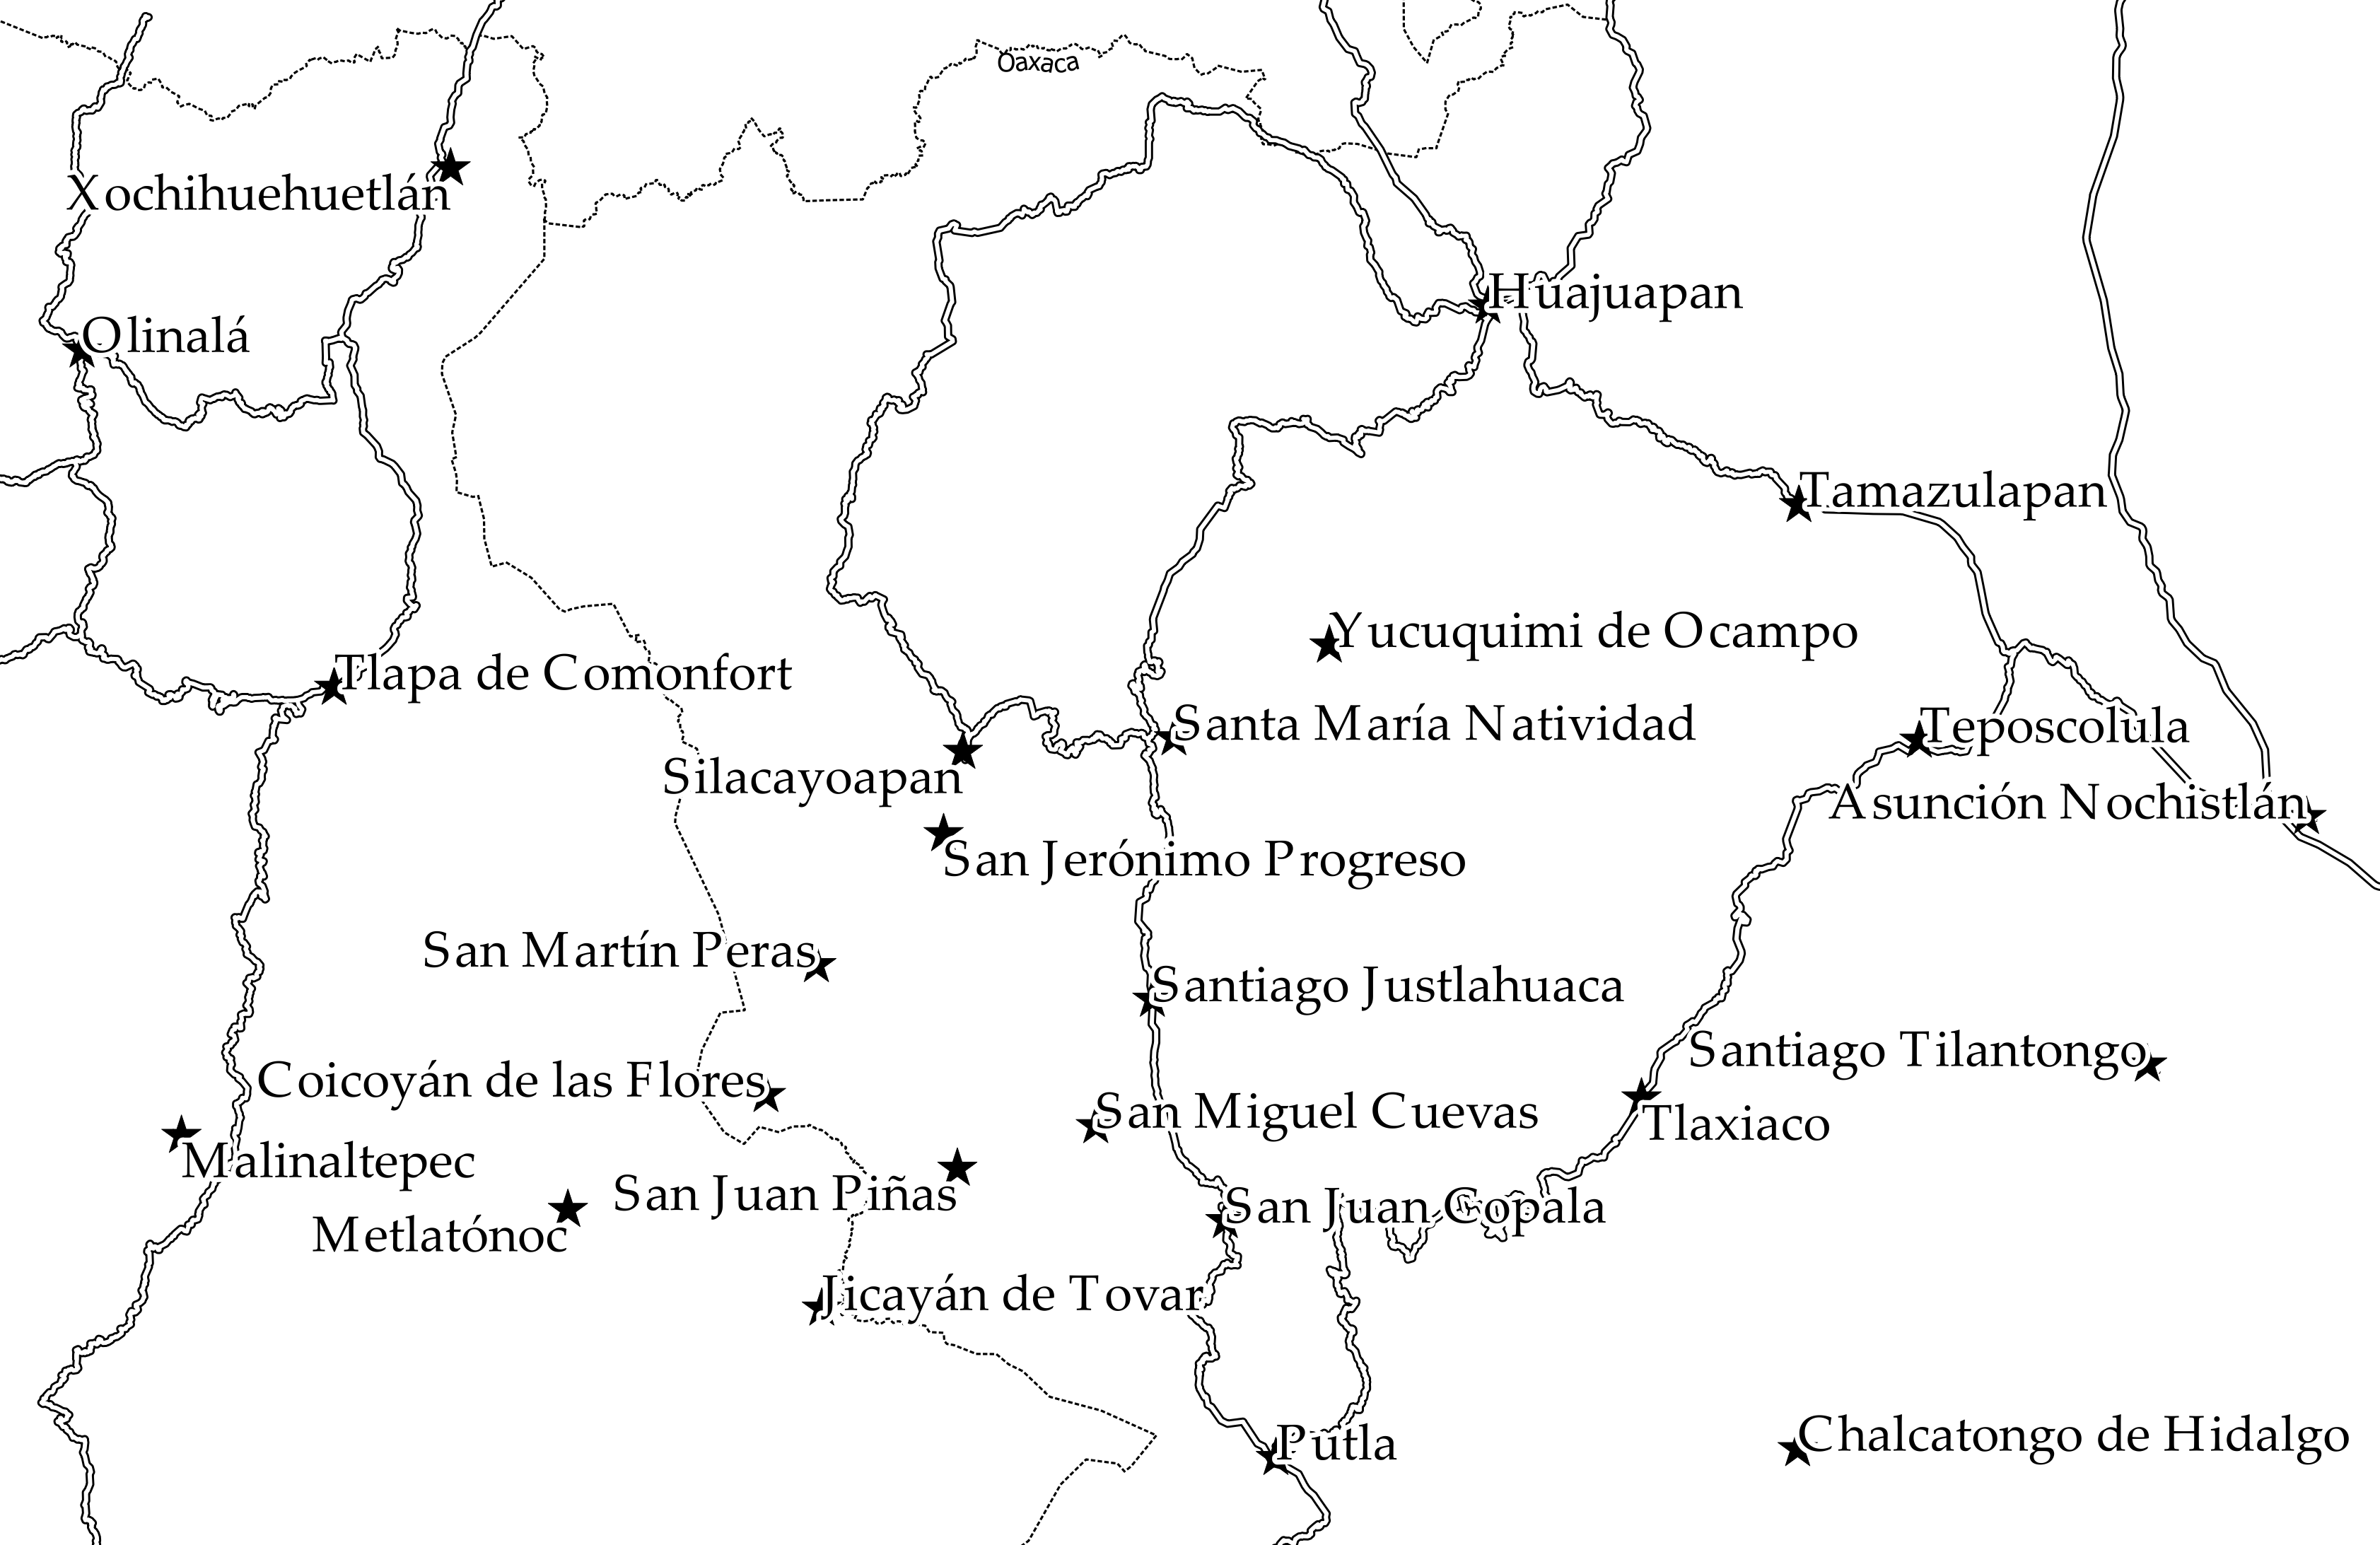
\includegraphics[width=\textwidth]{figures/mixteca4.png}
}
}%
\caption{San Miguel Cuevas in northwest Oaxaca (personal elaboration)}
\label{fig:cisneros:1}
\end{figure}

This paper concentrates on data from \il{Mixtec!Cuevas Mixtec}Cuevas Mixtec, the particular variant of \ili{Mixtec} spoken in the village of San Miguel Cuevas, or \textit{\~n\=u\=u$\star$ n\`u\`u$\star$ y\=uk\`u}\footnote{The stars here are introduced later as marking the presence of floating tones.} `the village on the mountain' as it is named in the variant.  This village is located in the municipality (or \textit{municipio}) of Santiago Juxtlahuaca, southwest of the municipal seat (Figure \ref{fig:cisneros:1}).  This location might put \il{Mixtec!Cuevas Mixtec}Cuevas Mixtec in \citegen{Josserand1983} classification as a variety of \il{Mixtec!Southern Lowlands Mixtec}Southern Lowlands Mixtec.  According to the 2010 Mexican Census, this village had a population of 522 inhabitants (242 male and 280 female) with 441 citizens over the age of three years of age that spoke an indigenous language (233 male and 208 female) (INEGI \citeyear{inegi2010}).  The local name for the variant of \ili{Mixtec} spoken here is \textit{t\`u'\=un nd\'a'v\'i} `poor language', although there is a movement to replace this manner of referring to the language with \textit{t\`u'\=un s\`av\`i} `rain language' or `Dzahui's language'.\footnote{\textit{Dzahui} is the name of the Mesoamerican rain deity that appears in \ili{Mixtec} codices and ancient stone carvings.  The movement to rename all \ili{Mixtec} languages as local translations of `rain language' or `Dzahui's language' has spread into much of the Mixteca region besides San Miguel Cuevas, though I have not been able to trace its origin or motivation.  Some motivation may come from the fact that the veneration of rain deities is a practice of the native \ili{Mixtec} religion which has survived the imposition of Catholicism in the colonial era.  In San Miguel Cuevas, there is a special stone named Saint Michael which is provided offerings in exchange for the prospect of rain.  I have also been told about a stone of similar purpose in Ixpantepec Nieves which has retained the name `rain' or \textit{Dzahui}.}  Due to early twentieth century educational policy against the retention of indigenous languages in Mexico, few \ili{Mixtec} speakers are trained in written forms of their languages \citep[29]{VelascoOrtiz2005}, and San Miguel Cuevas has yet to see a standardized, written form of theirs.

Beyond San Miguel Cuevas, speakers of this variant are also found in the United States, having immigrated to take on jobs in the service industry, manufacturing, and agriculture.  Most of these speakers are immigrants born in Mexico, and they are  located in Delaware, the Portland metropolitan area of Oregon, and Fresno county in California.  In Fresno, the speaker population is absorbed into the greater \ili{Mixtec} or Oaxacan community, which also has significant numbers of Mixtecs from Yucuquimi de Ocampo and Santiago Tilantongo in Oaxaca, and Metlat\'onoc and Jicay\'an de Tovar in Guerrero.  The variants of \ili{Mixtec} spoken by members of different towns may differ to the extent that \ili{Spanish} is preferred as a means of communication, and \il{Mixtec!Cuevas Mixtec}Cuevas Mixtec is therefore not widely spoken outside the home.  Within the home, \il{Mixtec!Cuevas Mixtec}Cuevas Mixtec is spoken more frequently to varying degrees.  Some local radio stations have accommodated some programming in several local varieties of \ili{Mixtec} at special times, though I am not certain that they have had programming in \il{Mixtec!Cuevas Mixtec}Cuevas Mixtec.  Local rap artist Miguel ``Una Isu'' Villegas has incorporated \il{Mixtec!Cuevas Mixtec}Cuevas Mixtec into the lyrics of several of his songs, and these songs are available on several media-sharing websites.

\subsection{Orthography of Cuevas Mixtec} \label{sec:cisneros:3.2}

For each example sentence of \ili{Mixtec} throughout this paper, I present the data with three transcription tiers: transcription, morpheme gloss, and translation.  Transcriptions are written using a variant of the official \ili{Mixtec} orthography endorsed by the Academy of the \ili{Mixtec} Language (\textit{Academia de la Lengua Mixteca} or \textit{Ve'e Tu'un Savi}), instead of phonetic symbols from the International Phonetic Alphabet (IPA).  This is intended to facilitate reading for \ili{Mixtec} scholars and other readers familiar with this orthography.  \tabref{tab:cisneros:1} presents the current alphabet for \il{Mixtec!Cuevas Mixtec}Cuevas Mixtec, with corresponding IPA symbols for each entry.  There are five oral vowels \textit{a e i o u}, voiceless affricate and plosives \textit{ch k ku p t ty},\footnote{The reader may notice that the letter \textit{u} is used for representing both a vowel and a secondary feature of two consonants \textit{ku} and \textit{ju}.  In the data, tone marking always occurs on vowel symbols, including those for /u/.  This distinguishes the occurrence \textit{u} as a vowel from its occurrences in consonant digraphs, which do not take tone marking.} voiced plosive \textit{d},\footnote{The voiced plosive \textit{d} seems to only occur on one pronoun and is likely an allophone of the voiceless plosive \textit{t}.} prenasalized stops \textit{mb nd ndy ng}, nasal stops \textit{m n \~n}, voiceless fricatives \textit{s sy x},\footnote{The plosive \textit{b} and the fricatives \textit{j ju} occur in loanwords and \isi{proper names} from \ili{Spanish}.} voiced fricatives \textit{v y}, and liquids \textit{l r}.\footnote{The tap \textit{r} seems to only occur in some pronouns and may be an allophone of \textit{ty}.}  There is additionally a glottal stop of ambiguous phonemic status, and this is written with an apostrophe.

\begin{table}[ht]
\caption{\il{Mixtec!Cuevas Mixtec}Cuevas Mixtec orthography and phone correspondences}
\label{tab:cisneros:1}
\begin{tabularx}{.5\textwidth}{CCCCCC} 
\lsptoprule
\textit{a} & \textit{b} & \textit{ch} & \textit{d} & \textit{e} & \textit{i}\\ 
/a/ & /b/ & /tʃ/ & /d/ & /e/ & /i/ \\
\midrule
\textit{j} & \textit{ju} & \textit{k} & \textit{ku} & \textit{l} & \textit{m}\\
/x/ & /xʷ/ & /k/ & /kʷ/ & /l/ & /m/\\
\midrule
 \textit{mb} & \textit{n} & \textit{nd} & \textit{ndy} & \textit{ng} & \textit{ñ}\\ 
/ᵐp/ & /n/ & /ⁿt/ & /\textsuperscript{ɲ}c/ & /\textsuperscript{ŋ}k/ & /ɲ/\\
\midrule
\textit{o} & \textit{p} & \textit{r} & \textit{s} & \textit{sy} & \textit{t}\\
/o/ & /p/ & /ɾ/ & /s/ & /ç/ & /t/\\
\midrule
\textit{ty} & \textit{u} & \textit{v} & \textit{x} & \textit{y} & \textit{'}\\
/c/ & /u/ & /β/ & /ʃ/ & /ʐ/ & /ʔ/\\
\lspbottomrule
\end{tabularx}
\end{table}

\ili{Otomanguean} languages are well known for the preponderance of suprasegmental features, and \il{Mixtec!Cuevas Mixtec}Cuevas Mixtec is no exception.  Nasalized vowels are represented with an adjacent \textit{n} as in \textit{an en in un}.   \il{Mixtec!Cuevas Mixtec}Cuevas Mixtec is also a highly tonal language, with three level tones that combine into nine possible contours.  High tones, low tones, and mid tones are marked with acute accent \textit{\'a}, grave accent \textit{\`a}, and macron \textit{\=a}, respectively.  With the help of more recent work on similar varieties of \ili{Mixtec} \citep{Carroll2015}, I have also been able to identify the presence of floating tones.\footnote{ Floating tones are applied to the first vowel of the following word, and their value depends on the tone value of the last vowel of the word they originate from.  They manifest as high tones when the tone of the last vowel is low and as low tones otherwise.  Therefore, the floating tone from \textit{n\`u\`u$\star$} `face' will be high, while the floating tone from \textit{ch\'it\'u$\star$} `cat' will be low.}  I have not thoroughly investigated the distribution of floating tones, so they are inconsistently marked in the data.  Where they are marked, the pending convention I have chosen is to represent their presence with a star $\star$. 

Many pronouns in the language have cliticized forms.  For clitics, I stray from the Academy of the \ili{Mixtec} Language and follow a convention observed in\linebreak \citegen{Bradley1988} \textit{Studies in the syntax of \ili{Mixtecan} languages} series by representing clitics as orthographically detached from host words.  The detachment is represented by horizontal space in the data, and therefore, no special marking for clitics is used.\footnote{The result of this convention is the lack of representation of data where clitics combine with truncated forms of host words.  Truncation often occurs on long vowels or [VʔV] strings after a clitic without a consonant is attached.}  Finally, the data itself throughout this paper is marked for acceptability as a phrase or sentence of the language, unacceptability, infelicity, and spontaneous elicitation.  Acceptable phrases and sentences are marked with a checkmark \checkmark, semantically or grammatically anomalous phrases are marked with an asterisk *, and infelicitous sentences are marked with a pound sign \#.  Spontaneously elicited phrases and sentences, or those which were produced by a speaker in speech or translation, are unmarked.

\subsection{Word order patterns of \il{Mixtec!Cuevas Mixtec}Cuevas Mixtec} \label{sec:cisneros:3.3}

This subsection covers basic word order patterns encountered in the language in order to facilitate reading of definiteness data later.  Basic sentence structure is presented first, and \il{Mixtec!Cuevas Mixtec}Cuevas Mixtec is shown to be a VSO language with certain conditions for optional or obligatory repositioning of verb arguments to a preverbal position.  Some aspects of the structure of the \is{noun phrases}noun phrase are presented afterwards in order to demonstrate the distribution of definite articles with respect to other modifiers later.  The subsection then presents examples of the distribution of \isi{noun classifiers}, which have occurrences as the \is{definite articles}definite articles of the language.

\subsubsection{Basic sentence structure} \label{sec:cisneros:3.3.1}

\il{Mixtec!Cuevas Mixtec}Cuevas Mixtec is a verb-initial language, like many languages of the \il{Mesoamerican languages}Mesoamerican area.  The subject argument of a verb consistently follows the verb if it is a clitic pronoun.  The object argument follows the subject in transitive sentences.
 
\ea[\checkmark]{\label{ex:cisneros:16}\il{Mixtec!Cuevas Mixtec}
\gll
k\'ix\`i \textbf{r\=a}\\
sleep.\textsc{ipfv} 3\textsc{sg.m}\\
\glt
`He is sleeping.'}
\z 

\ea[\checkmark]{\label{ex:cisneros:17}\il{Mixtec!Cuevas Mixtec}
\gll
k\'un\`i \textbf{r\'i} ty\`iku\`i\'i\\
want.\textsc{ipfv} 3\textsc{sg.aml} water\\
\glt
`It wants water.'}
\z 

Acceptable subject placement varies when the subject argument is not a clitic but a full nominal.  SVO word order is often the preferred word order for sentences with non-clitic subject arguments uttered without a \isi{discourse} context.\footnote{Example \REF{ex:cisneros:19} features a \isi{focus}-sensitive particle \textit{v\=a} which occurs in many other examples throughout the data.  It serves many roles such as emphasizer, restrictive/exclusive particle, and aspectual particle, similar to \ili{English} \textit{just}.  Its role in \REF{ex:cisneros:19} is uncertain, though speakers note that it is optional in this case.}  VSO word order in this case is often strange without a discourse context presented beforehand.\newpage

\ea \il{Mixtec!Cuevas Mixtec}\label{ex:cisneros:18}
Context: ∅
\ea[\checkmark]{
\gll
{\ob}\textbf{ty\`a} \textbf{Ju\'a\`an}{\cb} \`isy\=\i\=\i n {\ob}\=\i\=\i n k\'arr\'o{\cb}\\
{\db}the.\textsc{sg.m} Juan buy.\textsc{compl} {\db}one car\\
\glt
`Juan bought a car.'
}
\ex[\#]{
\gll
\`isy\=\i\=\i n {\ob}\textbf{ty\`a} \textbf{Ju\'a\`an}{\cb}  {\ob}\=\i\=\i n k\'arr\'o{\cb}\\
buy.\textsc{compl} {\db}the.\textsc{sg.m} Juan {\db}one car\\
\glt
(`Juan bought a car.')
}
\z 
\z

\ea \il{Mixtec!Cuevas Mixtec}\label{ex:cisneros:19}
Context: ∅
\ea[]{
\gll
{\ob}\textbf{ndy\=\i'\=\i} \textbf{v\=a} \textbf{n\=a}{\cb} \`isy\`i'\`i\\
{\db}all \textsc{foc} \textsc{3.hum} die.\textsc{compl}\\
\glt
`Everyone died.'}

\ex[\#]{
\gll
\`isy\`i'\`i {\ob}\textbf{ndy\=\i'\=\i} \textbf{v\=a} \textbf{n\=a}{\cb}\\
die.\textsc{compl} {\db}all \textsc{foc} \textsc{3.hum}\\
\glt
(`Everyone died.')
}
\z
\z

VSO word order becomes preferred with the addition of adverbial modifiers.  Temporal adverbs like \textit{\=\i k\=u} `yesterday' allow for non-clitic subjects to occur\linebreak postverbally without a \isi{discourse} context.

\ea[]{ \label{ex:cisneros:20}\il{Mixtec!Cuevas Mixtec}
Context: ∅  \\
\gll
\llap{\checkmark~}\=ik\=u \`isy\=\i\=\i n {\ob}\textbf{ty\`a} \textbf{Ju\'a\`an}{\cb}  {\ob}\=\i\=\i n k\'arr\'o{\cb}\\
yesterday buy.\textsc{compl} {\db}the.\textsc{sg.m} Juan {\db}one car\\
\glt
`Yesterday, Juan bought a car.'}
\z 

Wh-questions also confirm the basic word order to be VSO.  \il{Mixtec!Cuevas Mixtec}Cuevas Mixtec features obligatorily preposed wh-words in wh-questions.  Even if the wh-word is not a verbal argument, verbal arguments are unable to occur between the verb and the wh-word.

\ea \il{Mixtec!Cuevas Mixtec}\label{ex:cisneros:21}
\ea[\checkmark]{
\gll
ndy\'i\'i \`isy\=\i\=\i n {\ob}\textbf{ty\`a} \textbf{ju\'a\`an}{\cb} {\ob}\=\i\=\i n k\'arr\'o{\cb}\\
where buy.\textsc{compl} {\db}the.\textsc{sg.m} Juan {\db}one car\\
\glt
`Where did Juan buy a car?'
}

\ex[*]{
\gll
ndy\'i\'i {\ob}\textbf{ty\`a} \textbf{ju\'a\`an}{\cb} \`isy\=\i\=\i n {\ob}\=\i\=\i n k\'arr\'o{\cb}\\
where \phantom{[}the.\textsc{sg.m} Juan buy.\textsc{compl} \phantom{[}one car\\
\glt
(`Where did Juan buy a car?')
}
\z 
\z

There are some instances of a clitic pronoun co-occurring with a preverbal nominal as a coreferential item, similar to a \is{resumptive pronouns}resumptive pronoun or overt trace.

\ea \il{Mixtec!Cuevas Mixtec}\label{ex:cisneros:22}
\gll
{\ob}\textbf{ty\`a} \textbf{Ju\'a\`an}{\cb} \`isy\=\i\=\i n \textbf{r\=a} {\ob}\=\i\=\i n k\'arr\'o{\cb}\\
{\db}the.\textsc{sg.m} Juan buy.\textsc{compl} \textsc{3sg.m} {\db}one car\\
\glt
`Juan bought a car.'
\z 

This seems to indicate a sort of topicalization strategy, where the preverbal nominal occurs in a \isi{topic} position while the pronoun serves as the true verb argument.  There are three reasons for suggesting this proposal.  First, conjunction of sentences shows that preverbal subject arguments are restricted in their distribution when these resumptive pronouns occur.  A preverbal subject argument cannot occur for each conjunct sentence when the \is{resumptive pronouns}resumptive pronoun occurs in each.  If each conjunct sentence has a resumptive pronoun, the preverbal subject argument occurs once for the entire utterance, taking scope above the conjunction itself.  Preverbal subjects may occur within each conjunct sentence as long as there is no resumptive pronoun present. 

\ea \il{Mixtec!Cuevas Mixtec}\label{ex:cisneros:23}
\ea[*]{
\gll
{\ob}\textbf{ndy\=\i'\=\i} \textbf{v\=a} \textbf{n\=a}{\cb} sy\'it\=a \textbf{n\=a} ty\=a {\ob}\textbf{ndy\=\i'\=\i} \textbf{v\=a} \textbf{n\=a}{\cb} sy\'it\=asy\`a'\'a \textbf{n\=a}\\
{\db}all \textsc{foc} \textsc{3.hum} sing.\textsc{ipfv} \textsc{3.hum} and {\db}all \textsc{foc} \textsc{3.hum} dance.\textsc{ipfv} \textsc{3.hum}\\
\glt
(`Everyone sings, and everyone dances.')
}
\ex[\checkmark]{
\gll
{\ob}\textbf{ndy\=\i'\=\i} \textbf{v\=a} \textbf{n\=a}{\cb} {\ob}sy\'it\=a \textbf{n\=a} ty\=a sy\'it\=asy\`a'\'a \textbf{n\=a}{\cb}\\
{\db}all \textsc{foc} \textsc{3.hum} {\db}sing.\textsc{ipfv} \textsc{3.hum} and dance.\textsc{ipfv} \textsc{3.hum}\\
\glt
`As for everyone, they sing and dance.'
}
\ex[\checkmark]{
\gll
{\ob}\textbf{ndy\=\i'\=\i} \textbf{v\=a} \textbf{n\=a}{\cb} sy\'it\=a ty\=a {\ob}\textbf{ndy\=\i'\=\i} \textbf{v\=a} \textbf{n\=a}{\cb} sy\'it\=asy\`a'\'a\\
{\db}all \textsc{foc} \textsc{3.hum} sing.\textsc{ipfv} and {\db}all \textsc{foc} \textsc{3.hum} dance.\textsc{ipfv}\\
\glt
`Everyone sings and dances.'
}
\z 
\z

Secondly, there are certain types of modified nominals which would be barred from serving as topics as they are non-referential, such as negated nominals.  If a negated nominal occurs in the preverbal position, and it is interpreted as the sentence subject, a clitic subject cannot occur in the subject position after the verb(s).

\ea \il{Mixtec!Cuevas Mixtec}\label{ex:cosneros:24}
\gll
{\ob}\textbf{n\`i} \textbf{\=\i\=\i n} n\`a ty\`a\=a{\cb} k\'un\`i {\op}\textnormal{*}n\=a{\cp} k\=us\=u {\op}\textnormal{*}n\=a{\cp}\\
{\db}not.even one the.\textsc{hum} man want.\textsc{ipfv} \phantom{(*}3.\textsc{hum} sleep.\textsc{irr} \phantom{(*}3.\textsc{hum}\\
\glt
`No men wanted to sleep.'
\z 

\ea \il{Mixtec!Cuevas Mixtec}\label{ex:cisneros:25}
\gll
{\ob}\textbf{ch\'a\'a} n\`a ty\`a\=a{\cb} sy\'it\=a {\op}\textnormal{*}n\=a{\cp}\\
{\db}less the.\textsc{hum} man sing.\textsc{ipfv} \phantom{(*}3.\textsc{hum}\\
\glt
`Few men are singing.'
\z 

Thirdly, preverbal nominals are crucial for the expression of \is{genericity}generic statements.  Postverbal subject arguments force a progressive aspectual interpretation of the sentence below, while preverbal subject arguments allow for a \is{topic}topic-comment reading of the same material.  It is not crucial that the \is{resumptive pronouns}resumptive pronoun occur for triggering the topic-comment reading.

\ea \il{Mixtec!Cuevas Mixtec}\label{ex:cisneros:26}
\ea
\gll
sy\'e\'i {\ob}\textbf{ty\'i} \textbf{ch\'it\'u$\star$}{\cb} ty\`i\'in$\star$\\
eat.\textsc{ipfv} \phantom{[}the.\textsc{aml} cat mouse\\
\glt `The cat is eating mice.'

\ex
\gll
{\ob}\textbf{ty\'i} \textbf{ch\'it\'u$\star$}{\cb} sy\'e\'i {\op}r\'i{\cp} ty\`i\'in$\star$\\
{\db}the.\textsc{aml} cat eat.\textsc{ipfv} {\phantom{(}}3\textsc{sg.aml} mouse\\
\glt `The cat eats mice.'
\z 
\z

Without the resumptive pronoun, the sentence is interpreted as being an answer to a question.  This might suggest that preverbal arguments without co-occurring resumptive pronouns are \is{focus}focalized.

\subsubsection{Basic noun phrase structure}\is{noun phrases} \label{sec:cisneros:3.3.2}

\is{nouns}Nouns in \il{Mixtec!Cuevas Mixtec}Cuevas Mixtec do not require modification in order to occur as verb arguments.  They frequently occur in \is{bare nominals}bare forms and are often interpreted as \isi{indefinites} in such cases.

\ea \il{Mixtec!Cuevas Mixtec}\label{ex:cisneros:27}
\gll \textbf{ch\'it\'u$\star$} sy\'e\'i r\'i \textbf{ty\`i\'in$\star$}\\
cat eat.\textsc{ipfv} 3\textsc{sg.aml} mouse\\
\glt `Cats eat mice.'
\z 

Different classes of nominal modifiers occur before or after the nominal.  There are at least four classes of items which may occur prenominally: \isi{quantifiers}, \isi{numerals}, \is{definite articles}definite articles, and a specifier.  The specifier \textit{m\=\i\'i} serves as a reflexive when modifying a pronoun, as in the case of \textit{m\=\i\'i r\=a} `himself'.

\ea \il{Mixtec!Cuevas Mixtec}\label{ex:cisneros:28}
\gll
{\ob}ty\`a Ju\'a\`an{\cb} k\'un\`i r\=a {\ob}n\'a k\=us\=u \textbf{m\=\i\'i} r\=a{\cb}\\
{\db}the.\textsc{sg.m} Juan want.\textsc{ipfv} 3\textsc{sg.m} {\db}\textsc{comp} sleep.\textsc{irr} \textsc{spec} 3\textsc{sg.m}\\
\glt
`Juan wants that he himself sleep.'
\z

While modifying a nominal, the function of the specifier seems to be that of encoding \isi{focus}, or the presentation of the modified nominal as new information.

\ea \il{Mixtec!Cuevas Mixtec}\label{ex:cisneros:29}
\gll
{\ob}\textbf{m\=\i\'i} ty\`a Ju\'a\`an{\cb} s\'at\'at\'a\\
{\db}\textsc{spec} the.\textsc{sg.m} Juan heal.\textsc{ipfv}\\
\glt
`Juan is the one healing others.'
\z 

\ea[\checkmark]{ \label{ex:cisneros:30}\il{Mixtec!Cuevas Mixtec}
\gll
{\ob}\textbf{m\=\i\'i} ty\`in\=a{\cb} nd\'e'\=\i{}\\
{\db}\textsc{spec} dog bark.\textsc{ipfv}\\
\glt
`It is the dog barking.'
}
\z 

Quantifiers occur in a prenominal position.  The examples below include the \isi{quantifiers} \textit{ndy\=\i'\=\i} `all' and \textit{ch\'a\'a} `few'.


\ea \il{Mixtec!Cuevas Mixtec}\label{ex:cisneros:31}
\gll
{\ob}\textbf{ndy\=\i'\=\i} ty\`in\=a{\cb} nd\'e'\=\i\\
{\db}all dog cry.\textsc{ipfv}\\
\glt
`All dogs bark.'
\z 

\ea \il{Mixtec!Cuevas Mixtec}\label{ex:cisneros:32}
\gll
{\ob}\textbf{ch\'a\'a} ty\`in\=a{\cb} k\'um\'i nd\=a'\`a\\
{\db}few dog have.\textsc{ipfv} hand\\
\glt
`Few dogs have hands.'
\z 

\ea \il{Mixtec!Cuevas Mixtec}\label{ex:cisneros:33}
\gll
{\ob}\textbf{ndy\`iku\`i\'i} n\`i\`i{\cb} v\`a'\=a \=a\\
{\db}all salt good 3.\textsc{ina}\\
\glt
`All salt is good.'
\z 

Quantifiers do not seem to co-occur with the specifier.  This might suggest that both quantifiers and the specifier form a grammatical class.

\ea[*]{ \label{ex:cisneros:34}\il{Mixtec!Cuevas Mixtec}
\gll
{\ob}\textbf{m\=\i\'i} \textbf{ndy\=\i'\=\i} ty\`in\=a{\cb} nd\'e'\=\i\\
{\db}\textsc{spec} all dog cry.\textsc{ipfv}\\
\glt
(`It is all dogs that bark.')
}
\z 

Numerals also occur prenominally, though they differ from quantifiers in being able to co-occur with the specifier.  The examples below feature the \is{numerals|(}numeral \textit{\`u'\`un} `five'.

\ea[\checkmark]{ \label{ex:cisneros:35}\il{Mixtec!Cuevas Mixtec}
\gll
\`isy\=\i n\=\i{} r\=a {\ob}\textbf{\`u'\`un} \~n\`andy\=\i\=\i{}{\cb}\\
see.\textsc{compl} 3\textsc{sg.m} {\db}five sun\\
\glt
`He saw five suns.'
}
\z 

\ea[\checkmark]{ \label{ex:cisneros:36}\il{Mixtec!Cuevas Mixtec}
\gll
{\ob}\textbf{m\=\i\'i} \textbf{\`u'\`un} ty\`in\=a{\cb} nd\'e'\=\i{}\\
{\db}\textsc{spec} five dog cry.\textsc{ipfv}\\
\glt
`It is five dogs that are barking.'
}
\z 

Quantifiers differ amongst themselves in their capacity to co-occur with numerals.  The quantifier \textit{ndy\=\i'\=\i} `all' seems to be able to co-occur with numerals, but \textit{s\=av\=a} `half' cannot.

\ea \il{Mixtec!Cuevas Mixtec}\label{ex:cisneros:37}\il{Mixtec!Cuevas Mixtec}
\gll
\textbf{ndy\=\i'\=\i} \textbf{k\`um\`i} ty\`in\=a y\'o'\=o\\
all four dog here\\
\glt
`the four dogs here'
\z 

\ea[*]{ \label{ex:cisneros:38}\il{Mixtec!Cuevas Mixtec}
\gll
{\ob}\textbf{s\=av\=a} \textbf{\`usy\`i} ty\`in\=a{\cb} nd\'e'\=\i{}\\
{\db}half ten dog cry.\textsc{ipfv}\\
\glt
(`Half of the ten dogs are barking.')
}
\z 

The \is{quantifiers}quantifier \textit{ndy\=\i'\=\i} has the ability to syllabically reduce in cases where numerals co-occur, while reduction is not possible before a \is{bare nouns}bare noun.  This suggests that the item is not identical to other instances of the quantifier \textit{ndy\=\i'\=\i}.

\ea \il{Mixtec!Cuevas Mixtec}\label{ex:cisneros:39}
\gll
\textbf{ndy\=\i} \textbf{k\`um\`i} ty\`in\=a y\'o'\=o\\
all four dog here\\
\glt
`the four dogs here'
\z 

\ea \il{Mixtec!Cuevas Mixtec}\label{ex:cisneros:40}
\gll
{\ob}\textbf{ndy\=\i} \textbf{\`un\`a} ty\`a\=a{\cb} \`isy\`i'\`i\\
{\db}all eight man die.\textsc{compl}\\
\glt
`The eight men died.'
\z 

\ea \il{Mixtec!Cuevas Mixtec}\label{ex:cisneros:41}
\gll
{\ob}\textbf{ndy\=\i} \textbf{\`uv\`i} ty\`in\=a{\cb} nd\'e'\=\i\\
{\db}all two dog cry.\textsc{ipfv}\\
\glt
`The two dogs bark.'
\z 

\ea[*]{ \label{ex:cisneros:42}\il{Mixtec!Cuevas Mixtec}
\gll
\textbf{ndy\=\i} \textbf{\=\i s\=u}\\
all deer\\
\glt
(`all deer')
}
\z 

A large number of items may occur postnominally, including \isi{demonstratives} and \is{relative clauses}relative clauses.  The following example features a demonstrative \textit{k\'a\=a} `over there', which follows the nominal within the noun phrase.

\ea \il{Mixtec!Cuevas Mixtec}\label{ex:cisneros:43}
\gll
{\ob}ty\`a Ju\'a\`an{\cb} \`isy\=a'\`an r\=a {\ob}\~n\=u\=u$\star$ \textbf{k\'a\=a}{\cb}\\
{\db}the.\textsc{sg.m} Juan go.\textsc{compl} 3\textsc{sg.m} {\db}village over.there\\
\glt
`Juan went to the village over there.'
\z 
\is{noun phrases|}

\subsubsection{Noun classifiers and their functions} \label{sec:cisneros:3.3.3}\is{noun classifiers|(}

\il{Mixtec!Cuevas Mixtec}Cuevas Mixtec features a robust grammatical gender system which is exhibited through both its pronoun and noun classifier inventories.  Noun classifiers in \il{Mixtec!Cuevas Mixtec}Cuevas Mixtec are semi-pronominal items which explicate, and are sensitive to, the underlying system of grammatical gender in the language.  They are semi-pronominal because, unlike pronouns, they are typically not interchangeable with nominals.  They exhibit several grammatical functions in the grammar of the language, including at least their uses as \is{definite articles}definite articles and relative pronouns, as is shown in this subsection. \tabref{ex:cisneros:2} provides the inventory of noun classifiers in the language. They often phonotactically resemble their cliticized pronominal counterparts, but not in all cases.  These noun classifiers are not \is{uniqueness}unique to \il{Mixtec!Cuevas Mixtec}Cuevas Mixtec among \ili{Mixtec} languages, and one may find their analogues across the family.  They are called \textit{prestressed pronouns} in \citegen{Bradley1988} \textit{Studies in the syntax of \ili{Mixtecan} languages} series, where they are described for several very different varieties of \ili{Mixtec}.  The \ili{Mixtec} languages differ widely in the exact inventory of genders that are recognized grammatically.  \citet{Macri1983} observes the gender systems of six different \ili{Mixtec} varieties.  All of these varieties had masculine, feminine, and animal genders, though they differed in recognizing inanimate, youth, liquid, and sacred genders.

\begin{table}
\begin{tabularx}{.5\textwidth}{CCC} 
\lsptoprule
Gender & Classifier & Pronoun\\
\midrule
\textsc{m} & \textit{\textbf{ty\`a}} & \textit{r\=a} \\
\textsc{f} & \textit{\textbf{\~n\'a}} & \textit{\~n\'a} \\
\textsc{yth} & \textit{\textbf{t\=a}} & \textit{sy\=\i} \\
\textsc{hum} & \textit{\textbf{n\`a}} & \textit{n\=a} \\
\textsc{aml} & \textit{\textbf{ty\'i}} & \textit{r\'i} \\
\textsc{str} & \textit{\textbf{t\'u}} & \textit{d\'u} \\
\textsc{liq} & \textit{\textbf{ndr\'a}} & \textit{r\'a} \\
\textsc{ina} & \textit{\textbf{\~n\`a}} & \textit{\~n\=a} \\
\lspbottomrule
\end{tabularx}
\caption{Classifiers vs. pronouns}
\label{tab:cisneros:2}
\end{table}

The grammatical function of these classifiers that is of primary interest for this paper is their occurrences as \is{definite articles}definite articles, although their uses expand beyond these cases.  When occurring in the prenominal position, these items contribute a meaning of a \is{familiarity}familiar individual which satisfies the nominal description.  Since they encode gender, they show agreement constraints which bar a noun classifier\largerpage from modifying a \is{nouns}noun with a conflicting inherent gender.

\ea \il{Mixtec!Cuevas Mixtec}\label{ex:cisneros:44}
\gll
\textbf{ty\`a} ty\`a\=a\\
the.\textsc{sg.m} man\\
\glt
`the man'
\z 

\ea[*]{ \label{ex:cisneros:45}\il{Mixtec!Cuevas Mixtec}
\gll
\textbf{ndr\'a} ty\`a\=a\\
the.\textsc{liq} man\\
\glt
(`the man')
}
\z 

Among the prenominal modifiers, \isi{definite articles} are the most adjacent to the \is{nouns}noun.  They seem to be able to co-occur with all other prenominal items.  While co-occurring with \isi{quantifiers} or numerals, they explicate the formation of \is{partitives}partitive constructions.

\ea \il{Mixtec!Cuevas Mixtec}\label{ex:cisneros:46}
\gll
{\ob}s\=av\=a \textbf{ty\'i} \textbf{ty\`in\=a}{\cb} nd\'e'\=\i\\
{\db}half the.\textsc{aml} dog cry.\textsc{ipfv}\\
\glt
`Half of the dogs bark/are barking.'
\z 

\ea \il{Mixtec!Cuevas Mixtec}\label{ex:cisneros:47}
\gll
{\ob}\`uv\`i \textbf{n\`a} ty\`a\=a{\cb} ku\`an\=u'\`u\\
{\db}two the.\textsc{hum} man go.home.\textsc{ipfv}\\
\glt
`Two of the men went home.'
\z 

\ea \il{Mixtec!Cuevas Mixtec}\label{ex:cisneros:48}
\gll
{\ob}\`uv\`i \textbf{ty\'i} ty\`in\=a{\cb} nd\'e'\=\i\\
{\db}two the.\textsc{aml} dog cry.\textsc{ipfv}\\
\glt
`Two of the dogs bark.'
\z 

They even co-occur with whatever combinations of quantifier and \is{numerals|)}numeral are possible in the language.

\ea{\label{ex:cisneros:49}\il{Mixtec!Cuevas Mixtec}
\gll
{\ob}ndy\=\i{} \`uv\`i \textbf{n\`a} ty\`a\=a{\cb} \`isy\`i'\`i\\
{\db}all two the.\textsc{hum} man die.\textsc{compl}\\
\glt
`The two of the men died.'}
\z 

\ea \il{Mixtec!Cuevas Mixtec}\label{ex:cisneros:50}
\gll
{\ob}ndy\=\i{} \`uv\`i \textbf{ty\'i} ty\`in\=a{\cb} nd\'e'\=\i\\
{\db}all two the.\textsc{aml} dog cry.\textsc{ipfv}\\
\glt
`The two of the dogs bark.'
\z 

Noun classifiers prescriptively occur with \isi{proper names} to denote individuals, although they may be dropped from names in very casual speech.  Proper names without classifiers also refer to names themselves.

\ea \il{Mixtec!Cuevas Mixtec}\label{ex:cisneros:51}
\gll
{\ob}{\op}\textbf{ty\`a}{\cp} K\=orn\'el\'i\'o{\cb} k\'u\'u {\ob}ty\`a k\'a\=a{\cb}\\
\phantom{[(}the.\textsc{sg.m} Cornelio be.\textsc{ipfv} {\db}the.\textsc{sg.m} over.there\\
\glt
`That guy over there is Cornelio.'
\z 

\ea \il{Mixtec!Cuevas Mixtec}\label{ex:cisneros:52}
\gll
{\ob}ty\`a y\'o'\=o{\cb} n\=a\~n\'i r\=a \textbf{K\=orn\'el\'i\'o}\\
{\db}the.\textsc{sg.m} here be.called.\textsc{ipfv} 3\textsc{sg.m} Cornelio\\
\glt
`This guy is called Cornelio.'
\z 

In addition to \isi{nouns}, noun classifiers also modify \isi{adjectives}, functioning as nominalizers while \is{definiteness marking}encoding definiteness.  

\ea \il{Mixtec!Cuevas Mixtec}\label{ex:cisneros:53}
\gll
\textbf{\~n\`a} y\'o'\=o\\
the.\textsc{ina} here\\
\glt
`this one here'
\z 

\ea \il{Mixtec!Cuevas Mixtec}\label{ex:cisneros:54}
\gll
\textbf{\~n\`a} ku\'i\`i\\
the.\textsc{ina} green\\
\glt
`the green one'
\z 

This strategy of nominalization extends to verb phrases, forming what appear to be \is{relative clauses!light-headed}light-headed relative clauses.

\begin{exe}
\ex \label{ex:cisneros:55}
\gll
\textbf{\~n\`a} \`isy\=a'\=a {\ob}\~n\'a M\'ar\'i\'a{\cb} {\ob}n\`u\`u$\star$ r\=a{\cb}\\
the.\textsc{ina} give.\textsc{compl} {\db}the.\textsc{f} Maria {\db}face 3\textsc{sg.m}\\
\glt
`the one that Maria gave to him'
\end{exe}

They also serve as relative pronouns in the sense that they introduce a \is{relative clauses}relative clause which bears a full nominal head.  Agreement in gender between the relative pronoun and the \is{relative clauses}relative clause head remains just as important as between nominals and \is{definite articles}definite articles.

\ea \il{Mixtec!Cuevas Mixtec}\label{ex:cisneros:56}
\gll
t\=ut\=u \textbf{\~n\`a} \`isy\=a'\=a {\ob}\~n\'a M\'ar\'i\'a{\cb} {\ob}n\`u\`u$\star$ r\=a{\cb}\\
book the.\textsc{ina} give.\textsc{compl} {\db}the.\textsc{f} Maria {\db}face 3\textsc{sg.m}\\
\glt
`the book that Maria gave to him'
\z 

\ea \il{Mixtec!Cuevas Mixtec}\label{ex:cisneros:57}
\gll
{\ob}ty\`a Ju\'a\`an{\cb} \`isy\=\i'\=\i{} r\=a {\ob}ty\`iku\`i\'i \textbf{ndr\'a} \`i\`i$\star$ v\`a'\=a{\cb}\\
{\db}the.\textsc{sg.m} Juan drink.\textsc{compl} 3\textsc{sg.m} {\db}water the.\textsc{liq} \textsc{neg} good.\textsc{ipfv}\\
\glt
`Juan drank the water that was not good.'
\z

Full nominal heads in \is{relative clauses}relative clause structures may themselves take on \is{definite articles}definite articles while a relative pronoun occurs at the same time.  This shows that the two usages of noun classifiers as either definite articles and relative pronouns are grammatically distinct.

\ea \il{Mixtec!Cuevas Mixtec}\label{ex:cisneros:58}
\gll
{\ob}\textbf{\~n\`a} t\=ut\=u{\cb} \textbf{\~n\`a} \`isy\=a'\=a {\ob}\~n\'a M\'ar\'i\'a{\cb} {\ob}n\`u\`u$\star$ r\=a{\cb}\\
{\db}the.\textsc{ina} book the.\textsc{ina} give.\textsc{compl} {\db}the.\textsc{f} Maria {\db}face 3\textsc{sg.m}\\
\glt
`the book that Maria gave to him'
\z 

Lastly, \is{relative clauses}relative clauses may even occur on \isi{proper names} to serve as \is{relative clauses!non-restrictive}appositive relative clauses, as in the example below.

\ea \il{Mixtec!Cuevas Mixtec}\label{ex:cisneros:59}
\gll
{\ob}\textbf{ty\`a} Ju\'a\`an \textbf{ty\`a} k\'ut\'o\'o k\=a'v\=\i{}{\cb} ku\`a'\`a v\`a'\=a k\'a'v\=\i{} r\=a\\
{\db}the.\textsc{sg.m} Juan the.\textsc{sg.m} like.\textsc{ipfv} read.\textsc{irr} much good read.\textsc{ipfv} 3\textsc{sg.m}\\
\glt
`Juan, who likes reading, reads a lot.'
\z 

\section{Regular nominals and definiteness encoding} \label{sec:cisneros:4}\is{uniqueness|(}

This section presents the semantic evidence for one of two claims.  \il{Mixtec!Cuevas Mixtec}Cuevas Mixtec very much patterns with other languages displaying multiple strategies for encoding definiteness by associating those strategies with different notions of definiteness.  For many nominal items of the language, definite \isi{bare nominals} are interpreted as unique with respect to some domain or situation, while overt \is{definite articles}definite articles contribute an \is{anaphora}anaphoric element to the interpretation of the nominal.  This is shown by observing patterns in the choice of \isi{definiteness marking} strategy within the semantic environments of both \is{immediate situation}immediate and \isi{larger situation} uses, anaphoric uses, and \isi{bridging}.  Thus, \il{Mixtec!Cuevas Mixtec}Cuevas Mixtec displays the correspondence of bare form with uniqueness interpretation, and overt marking with \isi{familiarity} interpretation, that has been noted for other languages by \citet{Schwarz2013} and \citet{Jenks2015}.  Most nominals of the language pattern this way, encompassing predicates without clear semantic associations among themselves, such as creatures and buildings.  For this reason, it is assumed that these nominals represent a default in definiteness encoding, owing them the label of \textit{regular} nominals.

\subsection{Uniqueness with regular nominals} \label{sec:cisneros:4.1}

Regular nominals in their bare forms may be interpreted as uniqueness definites, and this is evidenced by the use of bare forms for various non-anaphoric purposes explained by \citet{Hawkins1978}. \is{bare nominals}Bare forms are the natural form of regular nominals for the expression of \isi{larger situation} definiteness, meaning that they are able to \is{definiteness marking}encode definiteness as characterized by reference to an entity uniquely identified within general world knowledge.  The word \textit{y\`o\`o} `moon' refers to a entity uniquely identified as a moon in most real world interactions, and it displays resistance to modification by a noun classifier.

\ea[\checkmark]{ \label{ex:cisneros:60}\il{Mixtec!Cuevas Mixtec}
\gll
{\ob}ty\`a ju\'a\`an{\cb} nd\'e'\'e r\=a {\op}\textnormal{\#}\textbf{\~n\`a}{\cp} y\`o\`o\\
{\db}the.\textsc{sg.m} Juan look.\textsc{ipfv} 3\textsc{sg.m} \phantom{(\#}the.\textsc{ina} moon\\
\glt
`Juan is looking at the face of the moon.'
}
\z 

\is{bare nouns}Bare nouns are also used for \is{immediate situation}immediate situation definiteness.  They encode reference to an entity whose description is unique with respect to contextual knowledge that is shared between interlocutors.  This is similar to \is{larger situation}larger situation definiteness in that uniqueness is anchored to a domain of shared knowledge, but it differs in that this domain is quite small, non-global, or situational.  Any particular dog is not unique on a global scale, but dogs can be unique relative to their owners, as in the case of a family dog.  Thus, the word \textit{ty\`in\=a} `dog' rejects modification by a noun classifier in the following example.\is{noun classifiers|)}

\ea \il{Mixtec!Cuevas Mixtec}\label{ex:cisneros:61}
Context: A family's dog has gone missing for a week.  A relative enters their house one day to find them cheerful and then proceeds to ask why they are suddenly happy. \\
\gll
\`indy\=\i k\'ok\=o\=o {\op}\textnormal{\#}\textbf{ty\'i}{\cp} ty\`in\=a\\
return.\textsc{compl} \phantom{(\#}the.\textsc{aml} dog\\
\glt
`The dog came home!'
\z 

The results are fairly replicable for many examples of localized uniqueness.  Churches are often unique to many villages in the Mixtec region of Mexico.  The word \textit{v\=e\~n\`u'\=u} `church' may not take a \is{definite articles}definite article assuming the context provided below.

\ea \il{Mixtec!Cuevas Mixtec}\label{ex:cisneros:62}
Context: A man is visiting a Mixtec village, many of which have one church. \\
\gll
\`isy\=\i n\=\i{} \`i {\op}\textnormal{\#}\textbf{\~n\`a}{\cp} v\=e\~n\`u'\=u\\
see.\textsc{compl} 1\textsc{sg} \phantom{(\#}the.\textsc{ina} church\\
\glt
`I saw the church.'
\z 

There is another usage not identified by Hawkins, though it is observed in more recent studies of definiteness.  So-called \is{weak definites}\textit{weak definites} \citep{Carlson2006} are actually neither unique nor \is{anaphora}anaphoric.  They are nominals which appear to take on \is{definiteness marking}definiteness marking without referring to specific individuals.  Below, the weak definite \textit{the hospital} seems to refer more to the situation of being in a hospital rather than being in a particular one.

\ea \il{Mixtec!Cuevas Mixtec}\label{ex:cisneros:63}
\textit{Every accident victim was taken to \textbf{the hospital}. {\op}John to Mercy Hospital, Bill to Pennsylvania Hospital, and Sue to HUP{\cp}} \citep[3]{Schwarz2014}
\z 

I have been able to identify at least one word, \textit{y\`a'v\=\i} `market', which constitutes a case of a \is{weak definites}weak definite.  In the example below, the word takes on a \is{bare nominals}bare form, without \is{definite articles}definite articles.

\ea \il{Mixtec!Cuevas Mixtec}\label{ex:cisneros:64}
Context: Five people leave a room and return, having each gone shopping at a different market. \\
\gll
{\llap{\checkmark~}}{\ob}ndy\=\i'\=\i{} v\=a n\=a{\cb} \`isy\=a'\`an \textbf{y\`a'v\=\i}\\
{\db}all \textsc{foc} 3.\textsc{hum} go.\textsc{compl} market\\
\glt
`All of them went to the market.'
\z

A final note concerning the encoding of uniqueness for regular nominals is that these nominals may not necessarily occur in bare forms for a uniqueness interpretation.  Modified nominals may also have uniqueness interpretations at least in the case of \is{partitives}partitive constructions.  The example below demonstrates that a \is{larger situation}larger situation definite like \textit{y\`o\`o} `moon' may retain its uniqueness interpretation while modified by the \is{quantifiers}quantifier \textit{s\=av\=a} `half'.  The resulting partitive construction is not interpreted as quantification over a group of moons, but quantification over portions of the unique moon with respect to Earth. 

\ea \il{Mixtec!Cuevas Mixtec}\label{ex:cisneros:65}
\gll
{\ob}ty\`a Ju\'a\`an{\cb} \`isy\=\i n\=\i{} r\=a {\ob}s\=av\=a \textbf{y\`o\`o}{\cb}\\
{\db}the.\textsc{sg.m} Juan see.\textsc{ipfv} 3\textsc{sg.m} {\db}half moon\\
\glt
`Juan saw half of the moon.'
\z 

This might suggest that uniqueness is interpretable within the complement of a quantifier.  If that is true, it would entail that uniqueness interpretations of bare nominals syntactically correspond to an embeddable phrasal projection of some sort, such as a \is{determiner phrases}determiner phrase.  However, the exact structural relationship between quantifiers and nominals in \il{Mixtec!Cuevas Mixtec}Cuevas Mixtec remains to be explained.

\subsection{Familiarity with regular nominals} \label{sec:cisneros:4.2}\is{familiarity|(}

Besides bare forms of nominals, definite descriptions are also formed with overt \is{definiteness marking}marking by means of the language's \is{definite articles}definite articles, but the occurrence of definite articles comes with an alternative set of functions.  Definite articles are somewhat awkward when occurring in semantic environments that suggest the \is{uniqueness|)}uniqueness of the definite description's referent, as shown previously.  Definite articles are much more preferred when used to indicate an \is{anaphora}anaphoric relationship with an antecedent nominal, corresponding to the interpretation of the definite description as familiar.\footnote{It is worth noting here that there is a bit of variation in judgment across generational lines about the use of \is{definite articles}definite articles.  The data here better reflects younger generational speech, which features broader usage of definite articles for creating \isi{anaphora}.  Older speakers seem to dislike definite articles on regular nominals, or are at least much pickier about when they are used.  This might indicate a diachronic shift in the use of definite articles from something other than familiarity, which might also coincide with the development of definite articles in \il{Mixtec!Cuevas Mixtec}Cuevas Mixtec.  To my knowledge, definite articles are rarely described for other \ili{Mixtec} variants.}  This would follow \citeauthor{Schwarz2009} and \citeauthor{Jenks2015}'s findings that languages which feature \isi{bare nominals} as definite descriptions in addition to overt \isi{definiteness marking} tend to reserve the overt marking for the expression of familiarity.  In the narrative below, the first sentence presents a character, Juan, who is visiting a library to obtain a book that he is searching for.  The two follow-up sentences are near identical in form, though they differ in their \is{anaphora}anaphoric properties due to the presence or absence of the \is{definite articles}definite article \emph{\~n\`a}.  The first follow-up sentence has a bare nominal \textit{l\'ibr\'u} `book' which is interpreted existentially under negation.  This follow-up then claims that there are no books at all at the library.  In contrast, the presence of the definite article in the second follow-up allows for continued comment on the book Juan was looking for, saying that it was absent from the library without comment on other books. 

\ea \il{Mixtec!Cuevas Mixtec}\label{ex:cisneros:66}
\gll
\`isy\=a'\`an {\ob}ty\`a Ju\'a\`an{\cb} b\=\i bl\=\i \=ot\'ek\'a t\'a\`an n\'a n\=\i'\`i r\=a {\ob}\=\i\=\i n l\'ibr\'u{\cb}\\
go.\textsc{compl} {\db}the.\textsc{sg.m} Juan library so \textsc{comp} obtain.\textsc{irr} 3\textsc{sg.m} {\db}one book\\
\glt
`Juan went to the library in order that he get a book.'

\il{Mixtec!Cuevas Mixtec}
\ea[]
{\gll
s\=u\=u k\`o\'o \textbf{l\'ibr\'u} \'ind\=a\`a k\'a\=a\\
but \textsc{neg} book located.\textsc{ipfv} over.there\\
\glt
`But there was no book there.'}

\ex[\checkmark]{
\gll
s\=u\=u k\`o\'o {\ob}\textbf{\~n\`a} \textbf{l\'ibr\'u}{\cb} \'ind\=a\`a k\'a\=a\\
but \textsc{neg} {\db}the.\textsc{ina} book located.\textsc{ipfv} over.there\\
\glt
`But the book was not there.'}
\z 
\z

Because only the second follow-up is a continued comment on the book in the first sentence, it is the \is{definite articles}definite article which creates the crucial \is{anaphora}anaphoric link.

It is not crucial for the speaker to be familiar with the identity of the individual denoted by the \is{definite nominals}definite nominal.  The speaker may invoke a definite article for creating anaphoric links between coreferential nominals if their referent is learned about from hearsay.  The narrative below introduces an unspecified turkey that can only be referred back to with the occurrence of the definite article \textit{ty\'i}.  The two follow-up sentences are both declarations of hearsay that a turkey was sick, though only the second followup sentence is felicitous because of the presence of the \is{definite articles}definite article.

\ea \il{Mixtec!Cuevas Mixtec}\label{ex:cisneros:67}
\gll
\`isy\=a'n\'i {\ob}ty\`a ju\'a\`an{\db} k\'ol\=o\\
kill.\textsc{compl} {\db}the.\textsc{sg.m} Juan male.turkey\\
\glt
`Juan killed a turkey.'

\ea[\#]{
\gll
k\'ach\'i n\=a \~n\`a k\'u'v\`i v\=a \textbf{k\'ol\=o}\\
say.\textsc{ipfv} 3.\textsc{hum} \textsc{comp} sick.\textsc{ipfv} \textsc{foc} male.turkey\\
\glt
`They say that a turkey was sick.'}

\ex[\checkmark]{
\gll
k\'ach\'i n\=a \~n\`a k\'u'v\`i v\=a {\ob}\textbf{ty\'i} \textbf{k\'ol\=o}{\cb}\\
say.\textsc{ipfv} 3.\textsc{hum} \textsc{comp} sick.\textsc{ipfv} \textsc{foc} {\db}the.\textsc{aml} male.turkey\\
\glt
`They say that the turkey was sick.'}
\z 
\z 

Again, the first follow-up sentence is bizarre, but this time because it is interpreted as an assertion about a different turkey.  The second follow-up sentence is interpreted as being about the same turkey, thanks to the presence of the \is{definite articles}definite article.

Definite articles may even occur on \isi{mass nouns}, where their presence similarly encourages the formation of an \is{anaphora}anaphoric link between the definite description and a coreferential antecedent.  The presence of the definite article allows a nominal to refer back to a particular collection of mass that was introduced before.  The following example introduces a patch of salt that is later commented further upon as being brown.

\ea \il{Mixtec!Cuevas Mixtec}\label{ex:cisneros:68}
\gll
\`isy\=\i k\=a {\ob}ty\`a Ju\'a\`an{\cb} n\`u\`u$\star$ n\`i\`i\\
walk.\textsc{compl} {\db}the.\textsc{sg.m} Juan on salt\\
\glt
`Juan walked on salt.'

\ea
\gll
y\=a'\=a v\=a {\ob}\textnormal{\#}{\op}\textbf{\~n\`a}{\cp} n\`i\`i{\cb}\\
brown \textsc{foc} \phantom{[\#(}the.\textsc{ina} salt\\
\glt
`The salt was brown.'
\z 
\z

An interesting effect is observed with overt \isi{definiteness marking} on \isi{mass nouns}.  The occurrence of the article encourages the interpretation of the nominal referent as being unitized in some manner, so as to distinguish a particular body of mass.  In the following example with introductory and followup sentences, the occurrence of the definite article turns out to be optional, but with distinct effects in the interpretation of the referent of \textit{ty\`iku\`i\'i} `water'.  The lack of the article forces the interpretation of the nominal's referent to be a greater collection of water that is salient within a situation and which may not altogether be a participant in the drinking event.  The occurrence of the \is{definite articles}article encourages an interpretation of the nominal's referent to be a delimited amount of water which is participating in the drinking event, such as from a bottle.

\ea \il{Mixtec!Cuevas Mixtec}\label{ex:cisneros:69}
\gll
{\ob}ty\`a Ju\'a\`an{\cb} \`isy\=\i'\=\i{} ty\`iku\`i\'i\\
{\db}the.\textsc{sg.m} Juan drink.\textsc{compl} water\\
\glt
`Juan drank water (of unspecified source).'

\ea
\gll
\`i\`i$\star$ v\`a'\=a \textbf{ty\`iku\`i\'i}\\
\textsc{neg} good.\textsc{ipfv} water\\
\glt
`The water (from the river or lake) was not good.'
\ex
\gll
\`i\`i$\star$ v\`a'\=a {\ob}\textbf{ndr\'a} \textbf{ty\`iku\`i\'i}{\cb}\\
\textsc{neg} good.\textsc{ipfv} {\db}the.\textsc{liq} water\\
\glt
`The water (from a bottle) was not good.'
\z 
\z 

This seems to be in line with the findings on definiteness in \il{Mixtec!Cuevas Mixtec}Cuevas Mixtec for \isi{count nouns}.  The first followup sentence appears to represent a case of \is{immediate situation}immediate situation definiteness, whereby the \is{bare nominals}bare nominal indicates a \is{uniqueness}unique individual relative to a situation.  The bare nominal must then refer to the \is{maximality}maximal amount of water given a situation, which is not identical to the amount of water that Juan drank.  The \is{definite articles}article allows the nominal to refer back to the unitized water that Juan had drank and can be further commented on.\is{familiarity|)}

\subsection{Bridging} \label{sec:cisneros:4.3}\is{bridging|(}

The last usage of definite descriptions to be addressed in this paper are cases of bridging.  For many examples of bridging, both bare nominals and nominals with definite articles may serve as \isi{anaphora} for a non-coreferential antecedent, but there are also some cases which demonstrate a clear preference for one strategy of \is{definiteness marking}definiteness encoding over the other.  It turns out that these special cases include those relationships between definite descriptions and their antecedents that were first outlined by \citet{Schwarz2009}, and \il{Mixtec!Cuevas Mixtec}Cuevas Mixtec patterns with other languages by invoking its strategies for \is{definiteness marking}marking \isi{uniqueness} or definiteness for the same cases.\footnote{Schwarz has reported on encountering some variation among speakers' intuitions regarding bridging examples, and I have found similar variation for these examples in \il{Mixtec!Cuevas Mixtec}Cuevas Mixtec.  However, speakers' intuitions regarding bridging examples vary specifically in the strength of preference for one definiteness marking strategy over optionality between the two.  They do not vary with respect to which strategy is preferred, and when intuitions are strongest, the findings in the data align with \citeauthor{Schwarz2009}'s and \citeauthor{Jenks2015}' findings in other languages.}  In this language, when there is a \is{part-whole relationship}part-whole relationship between the definite description and the antecedent, the \isi{definiteness marking} strategy of choice is the \is{bare nominals}bare nominal, which indicates uniqueness.  The following example has the definite description \textit{t\'u y\'e'\'e} `the door' in a part-whole relationship with the \is{indefinites}indefinite nominal \textit{\=\i\=\i n v\=e'\=e} `a house'.  The occurrence of the \is{definite articles}definite article \textit{t\'u} is dispreferred.

\ea \il{Mixtec!Cuevas Mixtec}\label{ex:cisneros:70}
\gll
\`isy\=\i\=\i n {\ob}ty\`a Ju\'a\`an{\cb} {\ob}\=\i\=\i n v\=e'\=e{\cb}\\
buy.\textsc{compl} {\db}the.\textsc{sg.m} Juan {\db}one house\\
\glt
`Juan bought a house.'

\ea
\gll
sy\`a\`a t\'a'v\`i v\=a {\ob}{\op}\textnormal{\#}\textbf{t\'u}{\cp} y\'e'\'e{\cb}\\
already broken.\textsc{ipfv} \textsc{foc} \phantom{[(\#}the.\textsc{str} door\\
\glt
`The door was broken.'
\z 
\z 

Also in line with observations from other languages, since the antecedent is not coreferential with the definite description, it need not even be an individual.  The antecedent can also be a situation that is introduced and which may naturally entail conditions such as the existence of certain \isi{kinds} of entities.  The example below has a definite description \textit{k\'arr\'o} `car' with an antecedent adverbial phrase \textit{t\'a'\=an s\'ak\=ak\=a} which introduces a situation of driving.  Note that the inclusion of the definite article sounds awkward to speakers in this case.

\ea \il{Mixtec!Cuevas Mixtec}\label{ex:cisneros:71}
Context: Juan has a strange hearing problem which causes him to go deaf or have selective hearing in special circumstances. \\
\gll
{\ob}t\'a'\=an s\'ak\=ak\=a ty\`a Ju\'a\`an{\cb} \`i\`i k\=uv\=\i{} t\=as\`o'\=o r\=a {\ob}{\op}\#\textbf{t\'u}{\cp} k\'arr\'o{\cb}\\
{\db}every.time drive.\textsc{ipfv} the.\textsc{sg.m} Juan \textsc{neg} can hear.\textsc{ipfv} 3\textsc{sg.m} \phantom{[(\#}the.\textsc{str} car\\
\glt
`Every time Juan drives, he cannot hear the car.'
\z 

The scenario presented in the adverbial phrase entails the existence of some vehicle to be driven within the event.  The car is interpreted as being part of the driving event, which perhaps induces the choice of the \is{bare nominals}bare form for the definite description.

Finally, when there is a producer-product relationship between the definite description and the antecedent, the preference of \isi{definiteness marking} strategy is the one of overt marking.  The example below presents a scenario of a purchased book which necessarily has an author.  Authors are not in \is{part-whole relationship}part-whole relationships with books but producer-product relationships with them, so the nominal \textit{\=a\=ut\'o\`or} `author' preferably takes on a \is{definite articles}definite article for association between the nominal's referent and an aforementioned book.

\ea \il{Mixtec!Cuevas Mixtec}\label{ex:cisneros:72}
\gll
{\ob}ty\`a Ju\'a\`an{\cb} \`isy\=\i\=\i n r\=a {\ob}\=\i\=\i n t\=ut\=u{\cb}\\
{\db}the.\textsc{sg.m} Juan buy.\textsc{compl} 3\textsc{sg.m} {\db}one book\\
\glt
`Juan bought a book.'

\ea
\gll
{\ob}\textnormal{\#}{\op}\textbf{ty\`a}{\cp} \=a\=ut\'o\`or{\cb} k\'u\'u r\=a {\ob}ty\`a \~n\=u\=u$\star$ n\`u\`u$\star$ y\=uk\`u{\cb}\\
\phantom{[\#(}the.\textsc{sg.m} author be.\textsc{ipfv} 3\textsc{sg.m} {\db}the.\textsc{sg.m} village face mountain\\
\glt
`The author was (one) from San Miguel Cuevas.'
\z 
\z 

As far as the data regarding regular nominals, \isi{definiteness marking} strategy, and interpretation are concerned, there are few surprises, if any.  The next section discusses cases of nominals which do stray from the patterns noted above, particularly by either overextending the usage of \is{definite articles}definite articles for expressing \isi{uniqueness} or completely barring modification by definite articles. \is{bridging|)}

\section{Internal variation in definiteness marking}\is{definiteness marking|(} \label{sec:cisneros:5}\is{language internal variation|(}

There are at least two other classes of nominal which do not display a pattern akin to that of the regular nominals described before.  These other classes of nominal are small when compared to regular nominals which display the overt correspondence between encoding strategy and notion of definiteness.  The \textit{irregular} nominals require the presence of an overt \is{definite articles}definite article for both uniqueness and \is{familiarity|(}familiarity interpretations.  The \textit{complex} nominals do not occur with definite articles, perhaps because they seem to have one already morphologically built in, and so their \is{bare nominals}bare forms serve for both uniqueness and familiarity interpretations.  \tabref{tab:cisneros:3} summarizes the general correspondences between definiteness marking strategy and interpretation for all three classes.

\begin{table}[h]\is{uniqueness}
\begin{tabularx}{.5\textwidth}{CCC} 
\lsptoprule
{Noun type} & {Uniqueness} & {Familiarity}\\
\midrule
Regular & * & \checkmark \\
Irregular & \checkmark & \checkmark \\
Complex & * & * \\
\lspbottomrule
\end{tabularx}
\caption{Presence of overt \is{definite articles}definite article according to usage}
\label{tab:cisneros:3}
\end{table}

The differences displayed by these other classes of nominal are shown by comparison with regular nominals in their distinct grammatical behavior with respect to some of \citegen{Hawkins1978} usages of definite articles.  These nominals display differences in the obligatoriness of the absence or presence of definite articles while undergoing \is{immediate situation}immediate situation uses, \is{larger situation}larger situation uses, and \is{anaphora}anaphoric uses.  Therefore, they reflect distinct styles of encoding either uniqueness or familiarity.  There are only a handful of examples of these classes of nominal that this paper is able to provide, and the exact size of each class is yet to be determined.

\subsection{Irregular nominals and definiteness encoding} \label{sec:cisneros:5.1}

While regular nominals display a predictable pattern of associating distinct notions of definiteness with distinct definiteness marking strategies, the distinction is not recognized in the \is{morphosyntax}morpho-syntax of irregular nominals.  Irregular nominals are so called because they differ from regular nominals in not exhibiting \is{bare nominals}bare forms as definite descriptions, or rather, they do not feature bare forms as \is{unique definites}uniqueness definites as with regular nominals.  While the strategy for the encoding of \isi{anaphoricity} remains identical among these two classes of nominals, irregular nominals extend the use of \is{definite articles}definite articles to also encode uniqueness.  For example, the word \textit{y\=\i v\=\i} `people' does not permit bare forms to serve as definite descriptions where other nominals can.  The sentences below present a context where a man named Juan is visiting a village and is surprised by the disappearance of its inhabitants.  In this case, \textit{y\=\i v\=\i} cannot take a bare form and must take a definite article in order for the sentence to be acceptable.

\ea \il{Mixtec!Cuevas Mixtec}\label{ex:cisneros:73}
\gll
{\ob}ty\`a Ju\'a\`an{\cb} \`isy\=a'\`an r\=a {\ob}\~n\=u\=u$\star$ k\'a\=a{\cb}\\
{\db}the.\textsc{sg.m} Juan go.\textsc{compl} 3\textsc{sg.m} {\db}village over.there\\
\glt
`Juan went to the village over there.'

\ea
\gll
s\=u\=u k\`o\'o n\=\i{} \`ind\=an\=\i'\`i r\=a {\ob}\textnormal{*}{\op}\textbf{n\`a}{\cp} y\=\i v\=\i{}{\cb}\\
but \textsc{neg} even find.\textsc{compl} 3\textsc{sg.m} \phantom{[*(}the.\textsc{hum} people\\
\glt
`But he did not find the people.'
\z 
\z 

A different result is reached if the irregular nominal is switched out for a regular nominal such as \textit{v\=e\~n\`u'\=u} `church'.  In a typical Mixtec village, there is one church dedicated to the local patron saint, whom the village also tends to be named after.  In this case, the nominal takes a \is{bare nominals}bare form because there is no previous mention of a church to serve as an antecedent for the \is{definite articles}definite article.

\ea \il{Mixtec!Cuevas Mixtec}\label{ex:cisneros:74}
\gll
{\ob}ty\`a Ju\'a\`an{\cb} \`isy\=a'\`an r\=a {\ob}\~n\=u\=u$\star$ k\'a\=a{\cb}\\
{\db}the.\textsc{sg.m} Juan go.\textsc{compl} 3\textsc{sg.m} {\db}village over.there\\
\glt
`Juan went to the village over there.'

\ea
\gll
s\=u\=u k\`o\'o n\=\i{} \`ind\=an\=\i'\`i r\=a {\ob}{\op}\textnormal{\#}\textbf{\~n\`a}{\cp} v\=e\~n\`u'\=u{\cb}\\
but \textsc{neg} even find.\textsc{compl} 3\textsc{sg.m} \phantom{[*(}the.\textsc{ina} church\\
\glt
`But he did not find the/a church.'
\z 
\z 

The inventory of irregular nominals is not very large at all, and they all seem to have an interesting semantic similarity.  \tabref{tab:cisneros:4} provides a list of the irregular nominals I have been able to recognize so far.

\begin{table}\il{Mixtec!Cuevas Mixtec}\il{English}
\begin{tabularx}{.5\textwidth}{CC} 
\lsptoprule
{Cuevas Mixtec} & {English}\\
\midrule
\textit{\textbf{y\=\i v\=\i}} &  \textit{people} \\
\textit{\textbf{ty\`a\=a}} & \textit{man} \\
\textit{\textbf{\~n\=a'\`a}} & \textit{woman} \\
\lspbottomrule
\end{tabularx}
\caption{Irregular nominals}
\label{tab:cisneros:4}
\end{table}

Notice that each nominal is a human predicate, such that the selection of predicates represented among the irregular nominals seems to be indicative of an animacy hierarchy.  It would appear that the most animate predicates, human predicates in this case, form a special class that exploits the definite article for further uses beyond what is typical within the language.  The influence of animacy hierarchies in grammar has been well documented \citep{Dahl1996}, and there are clear examples of its interaction with definiteness in languages as common as \ili{Spanish}.  For \il{Mixtec!Cuevas Mixtec}Cuevas Mixtec, there seems to be a particular relationship between animacy and \isi{uniqueness} in particular, which has been grammaticized in a way that treats unique members of the highest rank in animacy as if they were \is{familiarity|)}familiar. 

It is important to note that, despite the seeming obligatoriness of the definite article in the presence of irregular nominals, the definite article is only obligatory for the \is{definiteness marking}expression of definiteness.  These same nominals may occur with some other types of \isi{determiners} without the definite article, such as with certain \isi{quantifiers}.  Therefore, cases of definite articles on irregular nominals are not cases of prefixes.

\ea[\checkmark]{ \label{ex:cisneros:75}
\gll
{\ob}t\=a'\=an \textbf{\=\i\=\i n} \textbf{ty\`a\=a} ty\`a k\'um\'i \=\i\=\i n b\'urr\'u{\cb} k\'an\=\i{} r\=a r\'i\\
{\db}every one man the.\textsc{sg.m} have.\textsc{ipfv} one donkey hit.\textsc{ipfv} 3\textsc{sg.m} 3\textsc{sg.aml}\\
\glt
`Every man that has a donkey hits it.'}
\z 

There are even some environments where the irregular nominal may shed off any prenominal material.  The only environment where I have noticed this is that of the preverbal position while the nominal also takes a \is{relative clauses}relative clause.  The example below shows that the same nominal has an optional \is{definite articles}definite article in the preverbal position, but an obligatory article in the postverbal position.  Both the preverbal position and the \is{relative clauses}relative clause seem to be important for optionality of the definite article, and it is mysterious why this should be the case. 

\ea \il{Mixtec!Cuevas Mixtec}\label{ex:cisneros:76}
\ea
\gll
{\ob}{\op}\textbf{ty\`a}{\cp} ty\`a\=a \textbf{ty\`a} k\'ut\'o\'o k\=a'v\=\i{}{\cb} ku\`a'\`a v\`a'\=a k\'a'v\=\i{} r\=a\\
\phantom{[(}the.\textsc{sg.m} man the.\textsc{sg.m} like.\textsc{ipfv} read.\textsc{irr} much good read.\textsc{ipfv} 3\textsc{sg.m}\\
\glt
`The man who likes reading reads a lot.

\ex
\gll
 \=ik\=u ku\`a'\`a v\`a'\=a \`ik\=a'v\=\i{} {\ob}\textnormal{*}{\op}\textbf{ty\`a}{\cp} ty\`a\=a \textbf{ty\`a} k\'ut\'o\'o k\=a'v\=\i{}{\cb}\\
yesterday much good read.\textsc{compl} \phantom{[*(}the.\textsc{sg.m} man the.\textsc{sg.m} like.\textsc{ipfv} read.\textsc{irr}\\
\glt
`Yesterday, the man who likes reading read a lot.
\z 
\z

Generally, however, irregular nominals must take on definite articles if they do not co-occur with \isi{numerals} or when they occur in preverbal position.  They must even take on definite articles if they are modified by quantifiers.  Many nominals are able to occur in \is{partitives}partitive constructions without any modifying material besides the quantifier.  In such constructions, nominals actually tend to have \is{genericity}generic interpretations, at least if the modified nominal occurs in preverbal position.

\ea[\checkmark]{\label{ex:cisneros:77}
\gll
{\ob}s\=av\=a \textbf{ty\`in\=a}{\cb} nd\'e'\=\i\\
{\db}half dog cry.\textsc{ipfv}\\
\glt
`Half of dogs bark.'}
\z 

\ea[\checkmark]{\label{ex:cisneros:78}
\gll
{\ob}s\=av\=a \textbf{ty\`iku\`i\'i}{\cb} \`isy\=\i'\=\i{} {\ob}ty\`a Ju\'a\`an{\cb}\\
{\db}half water drink.\textsc{compl} {\db}the.\textsc{sg.m} Juan\\
\glt
`Juan drank half the water.'}
\z 

Unlike regular nominals, irregular nominals are incapable of occurring without the \is{definite articles}definite article in the same environment.

\ea \il{Mixtec!Cuevas Mixtec}\label{ex:cisneros:79}
\gll
{\ob}s\=av\=a \textnormal{*}{\op}\textbf{n\`a}{\cp} \textbf{ty\`a\=a}{\cb} k\'um\'i nd\=a'\`a\\
{\db}half \phantom{*(}the.\textsc{hum} man have.\textsc{ipfv} hand\\
\glt
(`Half of men have hands.')
\z 

It may be worth noting other cases of definite articles occurring on \is{unique definites}uniqueness definites beyond the class of irregular nominals, so  as to demonstrate the semantic complexity of interactions between definite articles and nominals more broadly.  There are some very special cases of definite articles occurring on regular nominals in order to make their referents more precise.  The example below presents a case where a definite article is used to specify a member of a pair of unique individuals, rather than encode \isi{familiarity}.  The word \textit{m\=art\'o\`on} `administrator' has only two possible referents in the village festival context, the male and female administrators.  The occurrence of definite articles allows for precision as to which of them is being referred to.  As a regular nominal, the word \textit{m\=art\'o\`on} has the capacity to occur in a \is{bare nominals}bare form as a uniqueness definite, but it also takes on the definite article only to make precise the gender of the referent. 

\ea \il{Mixtec!Cuevas Mixtec}\label{ex:cisneros:80}
\gll
\`isy\=a'\`an \`i n\`u\`u nd\'ut\'ut\'u {\ob}n\`a ndy\'a\'a ch\=u\=un{\cb}\\
go.\textsc{compl} 1\textsc{sg} where meet.\textsc{ipfv} {\db}the.\textsc{hum} mind.\textsc{ipfv} work\\
\glt
`I went to where the festival organizers were meeting.'

\ea
\gll
ty\=a k\`o\'o \textbf{m\=art\'o\`on} n\=\i{} \`isy\=o\=o\\
and \textsc{neg} administrator even there.be.\textsc{compl}\\
\glt
`But the administrators were not there.'

\ex
\gll
ty\=a k\`o\'o {\ob}\textbf{ty\`a} \textbf{m\=art\'o\`on}{\cb} n\=\i{} \`isy\=o\=o\\
and \textsc{neg} {\cb}the.\textsc{sg.m} administrator even there.be.\textsc{compl}.\\
\glt
`But the male administrator was not there.'
\z 
\z 

The example shows that definite articles serve many purposes beyond the formation of definite descriptions in the language.  Since they also encode gender, it seems possible for some regions of the grammar of \il{Mixtec!Cuevas Mixtec}Cuevas Mixtec to exploit this aspect of their meaning while ignoring their tendency to also encode \isi{familiarity}.  Altogether, the data present a picture of overt definiteness marking in this language that complicates the narrow pattern observed for regular nominals. 

\subsection{Complex nominals and definiteness encoding} \label{sec:cisneros:5.2}

The last category of nominals to be discussed here are what will be called complex nominals.  Complex nominals differ from both previously mentioned classes of nominal in that they are barred from taking on definite articles.  This may be due to the fact that, as \is{compounding}compounds, they already feature a sort of built-in noun classifier.  The only case of a complex nominal that this paper discusses is that of \textit{ty\`ax\`in\`i} `mayor', as in the example below, which shows the unacceptability of a \is{definite articles}definite article.  The word is a compound of a noun classifier \textit{ty\`a} and the word \textit{x\`in\`i} `head', such that they are inseparable in order to retain the meaning of `mayor'.  If the complex nominal is switched out for a regular nominal like \textit{m\=a\'estr\'o} `teacher' in the same example, the option of attaching a definite article becomes available.

\ea \il{Mixtec!Cuevas Mixtec}\label{ex:cisneros:81}
Context: There is a competition between the mayors of each village, followed by a separate competition between the teachers.

\ea
\gll
{\ob}{\op}\textnormal{*}ty\`a{\cp} \textbf{ty\`ax\`in\`i} ty\`a \`is\'ak\=an\'a'\`a{\cb} ku\`an\=u'\`u r\=a\\
\phantom{[(*}the.\textsc{sg.m} mayor the.\textsc{sg.m} win.\textsc{compl} go.home.\textsc{ipfv} 3\textsc{sg.m}\\
\glt
`The mayor that won went home.'

\ex
\gll
{\ob}{\op}ty\`a{\cp} \textbf{m\=a\'estr\'o} ty\`a \`is\'ak\=an\'a'\`a{\cb} ku\`an\=u'\`u r\=a\\
\phantom{[(}the.\textsc{sg.m} teacher the.\textsc{sg.m} win.\textsc{compl} go.home.\textsc{ipfv} 3\textsc{sg.m}\\
\glt
`The teacher that won went home.'
\z  
\z
 
As a nominal, the word may be modified with \isi{numerals} and \isi{indefinite articles} despite the \is{noun classifiers|(}noun classifier. Even with the constraint against the occurrence of definite articles, complex nominals may still occur as \is{familiar definites}familiarity definites.  In the second sentence below, the nominal \textit{ty\`ax\`in\`i} `mayor' has the interpretation of referring to the same mayor that was previously mentioned.

\ea \il{Mixtec!Cuevas Mixtec}\label{ex:cisneros:82}
\gll
{\ob}ty\`a ju\'a\`an{\cb} \`ind\=at\'u'\'un r\=a sy\'i'\'in {\ob}\=\i\=\i n \textbf{ty\`ax\`in\`i}{\cb}\\
{\db}the.\textsc{sg.m} Juan chat.\textsc{compl} 3\textsc{sg.m} with {\db}one mayor\\
\glt
`Juan chatted with a mayor...'

\ea
\gll
ty\=a \textbf{ty\`ax\`in\`i} \`ik\=us\`i\`i \=\i n\=\i{} r\=a\\
and mayor cheerful.\textsc{compl} inside 3\textsc{sg.m}\\
\glt
`and the mayor was happy.'
\z 
\z 

The rejection of definite articles for these items may have an explanation in the occurrence of a derivationally built-in noun classifier \textit{ty\`a}. \is{compounding}Compounding with classifiers occurs quite commonly across \ili{Mixtec} and other \ili{Otomanguean} languages, though it is better understood as a diachronic phenomenon which has resulted in fossilized forms of classifiers \citep{Macri1983}.  Classifiers in compounds, or so-called \is{classifiers}\textit{lexical classifiers}, are distinct from the grammatically active noun classifiers for all \ili{Mixtec} languages.  They constitute a much larger inventory with meaning contributions that have been lost over time, and not all words of the language feature them.  Lexical classifiers may co-occur with \is{definite articles}definite articles, substantiating the claim that they are a distinct class of fossilized forms.

\ea \il{Mixtec!Cuevas Mixtec}\label{ex:cisneros:83}
\gll
ty\'i \textbf{ty\`i}-x\'u'\`u\\
the.\textsc{aml} \textsc{clf}-money\\
\glt
`the goat'
\z 

In addition, the noun classifier is actually interchangeable with other noun classifiers, in particular the plural human classifier \textit{n\`a}.  This allows the nominal to take on a plural \isi{number} meaning in what seems to be the only case of nominal inflection in this language.  Likewise, this item is still unable to co-occur with a definite article.

\ea \il{Mixtec!Cuevas Mixtec}\label{ex:cisneros:84}
Context: There is a gathering of villages. \\
\gll
{\ob}s\=av\=a {\op}\textnormal{*}n\`a{\cp} \textbf{n\`ax\`in\`i}{\cb} k\'u'v\`i n\=a\\
{\db}half  \phantom{(*}the.\textsc{hum} mayors sick.\textsc{ipfv} 3.\textsc{hum}\\
\glt
`Half the mayors were sick.'
\z 

Therefore, the classifier that occurs in the complex nominal is not quite the same as the lexical classifiers that have been more widely described for \ili{Mixtec} languages.  

Beyond etymological considerations, the rejection of definite articles could also be explained from a semantic point of view.  Mayors are of course \isi{relational nouns}, or designations dependent on an individual's relationship with something else.  For someone or something to be a mayor, there must be a town for that individual to be a mayor of, perhaps automatically inducing a \isi{bridging} environment with a \is{part-whole relationship}part-whole relationship.  Further investigation on other relational nouns would be necessary to substantiate this.  It does seem to be the case that true relational nouns such as body parts also reject modification by definite articles.  In contrast, body parts differ from \textit{ty\`ax\`in\`i} in that they seem to be be averse to occurrences as \isi{bare nominals} and require at least some other form of modification.

\ea \il{Mixtec!Cuevas Mixtec}\label{ex:cisneros:85}
Context: A teacher is overseeing a boy make a drawing of a man.  The teacher takes a look at the boy's progress, and notices that the head of the man is drawn disproportionately large.\\
\gll
k\'a'n\=u ndy\'a'\=a {\op}\textnormal{*}\textbf{\~n\`a}{\cp} x\`in\`i \textnormal{\#}{\op}r\=a{\cp}\\
big very \phantom{(*}the.\textsc{ina} head \phantom{\#(}3\textsc{sg.m}\\
\glt
`The head is too big.'
\z 

The complex nominal therefore presents another challenge to the development of a homogenous account of definiteness in \il{Mixtec!Cuevas Mixtec}Cuevas Mixtec.  There seems to be an active grammatical role that the noun classifier plays in the construction of a \is{relational nouns}relational noun such as `mayor' while avoiding the typical usage of \is{noun classifiers|)}noun classifiers as encoding \isi{familiarity} as definite articles.
The data in this section also presented the case of obligatory definite articles on irregular nominals for cases where regular nominals would be \is{bare nominals}bare, demonstrating the apparent influence of an animacy hierarchy on the distribution of definite articles.  The existence of both classes of nominal complicates an account of definiteness encoding strategy as uniformly corresponding to the expression of either \is{uniqueness|(}uniqueness or familiarity for \il{Mixtec!Cuevas Mixtec}Cuevas Mixtec.\is{language internal variation|)}\is{definiteness marking|)}

\section{Conclusion} \label{sec:cisneros:6}

This paper served as an presentation of the internal variation exhibited within \il{Mixtec!Cuevas Mixtec}Cuevas Mixtec with respect to strategies of definiteness marking, and what that variation may be the result of.  The data support the findings of \citet{Schwarz2009,Schwarz2013} and \citet{Jenks2015} that languages which feature distinct strategies for definiteness marking will often associate those strategies with distinct notions of definiteness.  One strategy will correspond to the expression of uniqueness, or the function of referring to an individual that uniquely fulfills the description provided by the noun.  Another strategy will correspond to (strong) familiarity, or the function of creating an \isi{anaphor} to previous linguistic expression in a \isi{discourse}.  \citet{Schwarz2013} and \citet{Jenks2015} found that in many languages which feature bare nominal definite descriptions in addition to overt definiteness marking, bare \is{definite nominals}definite nominals will be interpreted as \is{uniqueness}unique, while familiarity requires the overt marking.  The pattern is replicated in \il{Mixtec!Cuevas Mixtec}Cuevas Mixtec, which has \isi{bare nominals} serve as \is{unique definites}uniqueness definites in many contexts, and requires the occurrence of overt definite articles for the expression of familiarity.  This was shown by observing the grammatical constraints on definite descriptions within different semantic environments listed by \citet{Hawkins1978}.  Bare definites are preferred in cases of \is{larger situation}larger situation and \is{immediate situation}immediate situation uses of definite descriptions, environments which reinforce the uniqueness of the definite description's referent.  Nominals with overt \is{definite articles}definite articles were preferred in cases where the definite description was used as an \isi{anaphor}, corresponding to the \isi{familiarity} characterization of definite descriptions in the literature.  Even the case of \isi{bridging} demonstrated the predicted correspondences between relationship type and preferred strategy of definiteness marking.  Where the relationship between the definite description and its antecedent was a \is{part-whole relationship}part-whole relationship, the \is{bare nominals}bare form seemed to be preferred.  Where the relationship between the definite description and its antecedent was a producer-product relationship, modification by overt definite articles seemed to be preferred.

In contrast, the pattern explained above is only reserved for a large subset of the nominal inventory of \il{Mixtec!Cuevas Mixtec}Cuevas Mixtec.  There are smaller classes of nominal which either lack the capacity to occur in bare forms for most contexts, or lack the capacity to take on definite articles.  Those nominals that cannot shed the \is{definite articles}definite article were called \textit{irregular nominals}, and they appear to retain the capacity to express uniqueness despite the presence of the article.  Irregular nominals were shown to retain the definite article in \is{immediate situation}immediate situation uses of definite descriptions, and unable to shed them even in the presence of other modifiers such as \isi{quantifiers}.  The definite article was shown not to be a prefix because there are environments where it may disappear, such as when a \is{numerals}numeral occurs in its place.  All of the irregular nominals seem to be predicates of humanity of some sort, meaning `man', `woman', or `people'.  The data therefore suggest an interaction between overt definiteness marking, especially uniqueness marking, and an animacy hierarchy.  Irregular nominals contrast with complex nominals, which seem to not take definite articles at all.  Complex nominals included the \is{relational nouns}relational noun `mayor', which more frequently undergoes uses as a \is{uniqueness|)}\is{unique definites}uniqueness definite.  Examples of complex nominals are difficult to encounter, so a much more thorough study of this class is necessary to determine all the semantic properties involved in the inventory.  Ultimately, the data show that if we are to assume an account of the semantics of definiteness along the lines of \citeauthor{Schwarz2009} and \citeauthor{Jenks2015}, there must also be some account for the nominal contribution in how \isi{definiteness marking} preferences are determined.

\section*{Acknowledgements}

I would like to thank Miguel ``Una Isu'' Villegas, Leoncio V\'asquez-Santos, and Rufino Dominguez-Santos for their time and patience during elicitation and their excellent assistance and insight on aspects of \il{Mixtec!Cuevas Mixtec}Cuevas Mixtec grammar.  I would also like to thank the following people for their guidance or recommendations concerning research on the topic of definiteness: Florian Schwarz, Anastasia Giannakidou, Itamar Francez.  I would lastly like to thank those who have helped me put this paper together, by proofreading it or otherwise: George Borawski, the editors of this volume, and anonymous reviewers.  Finally, kudos to Ana Aguilar-Guevara, Julia Pozas, and Violeta V\'asquez-Rojas for putting together a terrific conference and making this volume possible.  This material is based on work supported by the National Science Foundation Graduate Research Fellowship Program under Grant No. DGE-1144082.  I am responsible for any errors that appear in this work.

\section*{Abbreviations}
\begin{multicols}{2}
	\begin{tabbing}
		\textsc{aml}\hspace{1em} \= animal \kill
		\textsc{hum} \> plural human \\
		\textsc{ina} \> inanimate \\
		\textsc{liq} \> liquid \\
		\textsc{spec} \> specifier \\ 
		\textsc{str} \> plant/structure \\
		\textsc{yth} \> youth \\
	\end{tabbing}
\end{multicols}

{\sloppy
\printbibliography[heading=subbibliography,notkeyword=this]
}
\end{document}